%\documentclass[12pt,oneside]{fithesis2}		% pc version
\documentclass[a4paper, 12pt, twoside]{fithesis2}		% print version

% ===== LOADING PACKAGES =====
% language settings, main documnet language last
\usepackage[english]{babel}
% enabling new fonts support (nicer)
\usepackage{lmodern}
% setting input encoding
\usepackage[utf8]{inputenc}
% setting output encoding
\usepackage[T1]{fontenc}
% fithesis2 requires csquotes
\usepackage{csquotes}
% set page margins
%\usepackage[top=3.0cm, bottom=3.5cm, left=2.4cm, right=2.4cm]{geometry}	% pc version
\usepackage[top=3.0cm, bottom=3.5cm, left=2.9cm, right=1.9cm]{geometry}	% print version
% package to make bullet list nicer
\usepackage{enumitem}
% math symbols and environments
\usepackage{mathtools}
\usepackage{amsmath}
% packages for complex tables
%\usepackage{tabularx}
%\usepackage{multirow}
%\usepackage{dcolumn}
%\usepackage{array}
% package for defining new floating environments
\usepackage{float}
\usepackage[labelfont=]{caption}
%\usepackage{newfloat}
% package for drawing
\usepackage{tikz}
\usetikzlibrary{shapes,positioning,fit}
% code listings
\usepackage{listings}
%\usepackage{verbatim}

% indentation
% vertical space between paragrahps, no indentation
%\usepackage[parfill]{parskip}  % TODO: nefunguje -> zfunkcnit (ale asi je to tak dobre, maji to tak vsici)
% space between paragraphs
\setlength{\parskip}{0.6em plus0.2em minus0.2em} % zkraceni vzdalenosti mezi odstavci

% bibliography management
\usepackage[backend=biber, 		% use biber as backend instead of BiBTeX
        %dashed=false                    % when there is an author twice, still write his/her name
	bibstyle=ieee-alphabetic, 	% bibliography style: IEEE with alphabetic citations
	citestyle=alphabetic, 		% citation style
	url=true, 			% display urls in bibliography
	hyperref=auto,			% detect hyperref and create links
	%block=ragged, 			% format bibliography into blocks, ragged on right
]{biblatex}
\addbibresource{thesis.bib}

% setting custom colors for links
\usepackage{xcolor}
\definecolor{dark-red}{rgb}{0.6,0.15,0.15}
\definecolor{dark-green}{rgb}{0.15,0.4,0.15}
\definecolor{medium-blue}{rgb}{0,0,0.5}
\definecolor{light-gray}{rgb}{0.93,0.93,0.93}
% generating hyperlinks in document
\usepackage{url}
\usepackage[plainpages=false, 	    % get the page numbering correctly
            pdfpagelabels, 	    % write arabic labels to all pages
            unicode,	 	    % allow unicode characters in links
            colorlinks=true, 	    % use colored links instead of boxed (pc version)
            %hidelinks, 		    % hide links (print version)
            linkcolor={dark-red},
            citecolor={dark-green},
            urlcolor={medium-blue}
			]{hyperref}

% ===== FI THESIS SETTINGS =====

\thesistitle{Automatic Question Generation\\and Adaptive Practice}
\thesissubtitle{Bachelor thesis}
\thesisstudent{Tomáš Effenberger}
\thesiswoman{false}
\thesisfaculty{fi}
\thesisyear{spring 2015}
\thesisadvisor{RNDr.\ Jan Rygl}
\thesislang{en}

% ===== LATEX DOCUMENT SETTINGS =====

% only put chapters and sections into the TOC
\setcounter{tocdepth}{2}   % nefunguje (podle navodu by melo fungovat s 1, ale neni tomu tak)


% adjusting hyphenation penalties
%\tolerance=10000
%\hyphenpenalty=500

% hyphenations settings
\hyphenation{DBpedia}

% renew command for shorter and nicer underscore
\renewcommand{\_}{\leavevmode \kern0.07em\vbox{\hrule width0.4em}}


% ===== COMMANDS =====

%--------------------------------------------------------------------
% define square symbol
%--------------------------------------------------------------------
\newcommand{\squarebullet}{\textcolor{black}{\raisebox{0.15em}{\rule{4pt}{4pt}}}}

%--------------------------------------------------------------------
% define new itemize environment with squares and smaller spaces
%--------------------------------------------------------------------
\newenvironment{myItemize}{
  \begin{itemize}[leftmargin=2em,rightmargin=1em,itemsep=\parskip ,parsep=0em,topsep=0em,partopsep=0em]
  \renewcommand{\labelitemi}{\squarebullet}
  \renewcommand{\labelitemii}{$\diamond$}
}{
  \end{itemize}
}

\newenvironment{myEnumerate}{
  \begin{enumerate}[leftmargin=2em,rightmargin=1em,itemsep=\parskip ,parsep=0em,topsep=0em,partopsep=0em]
}{
  \end{enumerate}
}

%--------------------------------------------------------------------
% define new environment for Python code
%--------------------------------------------------------------------

%\lstset{%
%  language=SQL,%
%  morekeywords={PREFIX,LIMIT},%
%  basicstyle=\small\ttfamily,
%  frame=single%
%}

\lstnewenvironment{code}{%
  \lstset{backgroundcolor=\color{light-gray},
  frame=lines,
  %framerule=1pt,
  rulecolor=\color{black},
  basicstyle=\ttfamily,
  columns=fullflexible,
  showspaces=false,
  showstringspaces=false
  }}{}

%--------------------------------------------------------------------
% exercise environment
%--------------------------------------------------------------------
\newcounter{choice}
\renewcommand\thechoice{\Alph{choice}}
\newcommand\choicelabel{\thechoice.}

\newenvironment{choices}%
  {\vspace{0.8em}\list{\choicelabel}%
     {\usecounter{choice}\def\makelabel##1{\hss\llap{##1}}%
       \settowidth{\leftmargin}{W.\hskip\labelsep\hskip 0.01em}%
       \def\choice{%
         \item
       } % choice
       \labelwidth\leftmargin\advance\labelwidth-\labelsep
       \topsep=0pt
       \partopsep=0pt
     }%
  }%
  {\vspace{-0.7em}\endlist}

%\setlength{\abovecaptionskip}{25pt plus 3pt minus 2pt}
\floatstyle{boxed}
\newfloat{exercise}{thp}{exrcs}[chapter]
\floatname{exercise}{Exercise}

\newenvironment{question}
{
  \begin{center}
  \begin{tabular}{p{0.9\textwidth}}
  \vskip 0.05em
}
{
  \\
  \end{tabular}
  \end{center}
}

% gap in the sentence (bottom line)
\newcommand{\sentenceGap}{\rule{1.5cm}{0.4pt}~}

%--------------------------------------------------------------------

% ===== CHEAT SHEET =====

% == full width image

%\begin{figure}[b!]
%\centering
%\includegraphics[width=\textwidth]{images/bla.bla}
%\caption{bla bla bla}
%\label{fig:bla-bla}
%\end{figure}


% == myItemize

%\begin{myItemize}
%\item \textbf{Bla}\\
%  bla
%\item \textbf{Bla}\\
%  bla
%\item \textbf{Bla}\\
%  bla
%\end{myItemize}


% ===== BEGIN DOCUMENT =====
\begin{document}

\FrontMatter
\ThesisTitlePage

\begin{ThesisDeclaration}
\DeclarationText
\AdvisorName
\end{ThesisDeclaration}

\begin{ThesisThanks}

  TODO (Sir, NLP a ALG)
%I'd like to thank Petr for his guidance, enthusiasm and inspiring discussions.
%I also owe much to my mom and brother for their continuous support. Thank you.

%\noindent
%Further thanks goes to all my friends who had to put up with my enthusiasm
%and numerous research details they may have never asked for $\ddot\smile$.

%\noindent
%Last but not least, I'd like to acknowledge the Laboratory of Security and Applied Cryptography and
%the National Grid Infrastructure MetaCentrum for providing access to their computing and storage facilities.
\end{ThesisThanks}

\begin{ThesisAbstract}
When studying, it is more efficient not just to read about the topic, but also to practice the knowledge, e.g. by answering some multiple choice questions. Today, there is a huge amount of information to study (consider Wikipedia) and it is not possible to create a set of question for all topics manually. However, we can generate questions automatically, using techniques of artificial intelligence and natural language processing. This thesis explores the state-of-the-art approaches to question generation and describes their advantages and disadvantages. The thesis also suggests a design of the general framework for practicing knowledge from articles. This framework is implemented and publicly accessible through a web interface.
\end{ThesisAbstract}

\begin{ThesisKeyWords}
% TODO: profiltrovat na ty opravdu relevantni
knowledge representation, question generation, adaptive practice, learning,
multiple choice questions
%artificial intelligence, natural language processing,
\end{ThesisKeyWords}

\MainMatter
\tableofcontents

% ===========================  CHAPTER ===========================
\chapter{Introduction}
\label{chap:intro}

TODO: intro, goal of the thesis (dodelat podle oficialniho zadani / abstraktu)

Mere repeated reading of the text which one is traying to learn is unefficient method of learning, while answering to related questions leads to [better long-term knowledge / dlouhodobemu zapamatovani] \parencite{edu-improve}.

TODO: 2 ruzne cile: procvicovani (uceni) tematu vs. testovani; i pri procvicovani tematu muzu chtit i to testovani (abych vedel, jak na tom jsem) (budu se venovat obema (?) a v implementovanem systemu to bude nekde na pomezi)

TODO: neco o tom, ze vytvaret testy manualne je time-consuming, takze by bylo fajn to autmatizovat

In spite of active and [dlouhodoby nebo tak neco] research of question generation
(e.g. \parencite{questions-wolfe, questions-eval}) [mozna pridat dalsi, pripadne rozepsat - priklad early research a recent research],
there is still no publicly available web application to solve this task.
And I am sure that such application would be really useful. Typical example is to make self-studying more efficient by answering a few generated questions after reading an article to verify and consolidate the new knowledge.
[overit aktualnost a jasne urcit moment o kterem mluvim (neexistuje tady a ted)]

That is why I have implemented \textit{Smartoo, Smart Artificially Intelligent Tutor}, modular and extensible framework for question generation and adaptive practice
of knowledge from \emph{Wikipedia}%
\footnote{\url{http://en.wikipedia.org/}}
articles.
The Smartoo Framework is licensed under the GNU General Public License, version 2 [citovat?, licenci rozmyslet].
The source code is available from project's page on \textit{GitHub}.%
\footnote{\url{http://github.com/effa/smartoo}}
I have used the framework to create a simple [instance/demo/prototype?] of the web application for practicing knowledge from Wikipedia articles.%
\footnote{\url{http://smartoo.thran.cz}}

The whole practicing process consists of four steps.
First step is to extract facts from the given article.
Besides the knowledge extraction itself, knowledge representation is an important issue as well.
Extraction and representation of the knowledge is the topic of \autoref{chap:knowledge}.

In \autoref{chap:exercises}, excercises generation is discussed.
Usually, exercises will be just multiple choice questions, but other exercises types are possible as well.
In this step major concerns are: selection of a fact (or set of facts) from which the exercise will be generated, transformation from the fact (or facts) to the exercise and in case of multiple choice questions selection of good \textit{distractors} (incorrect choices).

TODO: upravit podle aktualniho rozdeleni na kapitoly: Although we could stop here and submit all generated questions to the user, it has been proven to be useful to make two more steps.
In \autoref{chap:exercises-grading}, I talk about exercises grading.
We can be interested in various parameters, such as difficulty, relevance to the article or probability that the question is gramatically [?].

Having the exercises graded, we can filter them and only present these with reasonable difficulty, relevance and correctness probability.
But again, we can introduce one more step to make learning more efficient -- adaptive practice.
According to the user performance, we can choose easier or more difficult questions. I talk about some common strategies for this task in \autoref{chap:practice}.

In \autoref{chap:smartoo}, I describe the Smartoo Framework in detail
and we will see how these four steps are transparently glued and how a component for each step should look like.
I also mention how each of the four components is implemented in the online prototype system.

Smartoo is designed to collect both implicit and explicit feedback from users.
I analyze feedback from about one month testing period in \autoref{chap:evaluation}.

Finally, in the \autoref{chap:future}, I present planned future development of Smartoo application.


%The thesis text was typeset in \LaTeX{} using the \textit{fithesis2} package created by Stanislav Filipčík \parencite{fithesis}.

%TODO: (?) The text of the thesis is licensed under a Creative Commons Attribution 3.0 Unported License.

[Maybe TODO: diagram kroku a vystupu (napr. aby bylo jasne, ze knowledge extraction je moznost, nikoliv nutnost)]



% ===========================  CHAPTER ===========================
\chapter{Knowledge Extraction and Representation}
\label{chap:knowledge}

Instead of creating exercises directly from the text in natural language (unstructured data),
one can at first attempt to extract the meaning from the text,
i.e. convert the text into the structured data.
This process is called \textit{information extraction} \cite[][262]{nlp-python}.
Information extraction has several subtasks, the two most relevant for us are:
\begin{myItemize}
  \item \textit{named entity recognition} -- extraction of terms (e.g. \textit{"Abraham Lincoln"}) and numeric expressions from the text,
\item \textit{relation recognition} -- extraction of relations between the entities.
\end{myItemize}

One way to create exercises is to first perform the relation extraction and then create the exercises from built structured knowledge representation. Another approach is to generate exercises from text with discovered named entities. We will take closer look at both these approaches in \autoref{chap:exercises}.


% ---------------------------  SECTION  ---------------------------
\section{RDF Graph}
\label{sec:rdf-graph}

There are many ways how to represent knowledge [Maybe TODO: zminit nejake ostatni].
One common way is to represent knowledge as a graph (\textit{knowledge graph}), where vertices are named entities
and edges indicate relations between the entities.
The most popular standardization of this approach recently became the \textit{RDF Graph}%
\footnote{RDF stands for \textit{Resource Description Framework}. [Maybe TODO: odkaz]}.
RDF graph is a collection of subject -- predicate -- object triples \parencite[][63]{semantic-web},
each triple is called a \textit{fact}. Simple example of a few facts about Alan Turing and Alonzo Church:

\begin{code}
Alan Turing - type - person
Alan Turing - birthdate - 23 June 1912
Alan Turing - nationality - British
Alan Turing - doctoral advisor - Alonzo Church
Alonzo Church - type - person
Alonzo Church - nationality - American
Alonzo Church - birthdate - 14 June 1903
\end{code}

\autoref{fig:simple-rdf-graph} shows how can be this collection of facts thought of as a directed graph.
Vertices corresponds to subjects and objects. Each fact maps to one edge, with direction from the subject to the object and with edge value given by the predicate.

\begin{figure}[h]
  \centering
  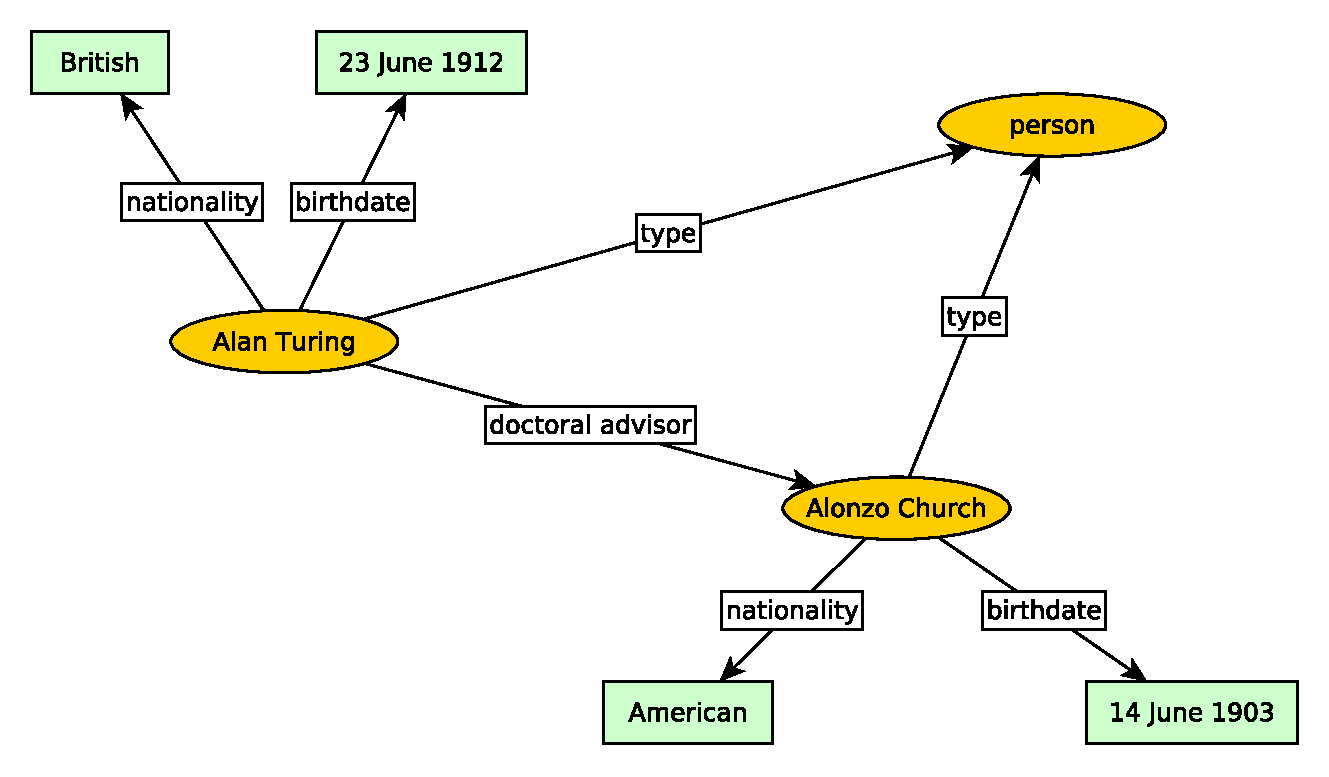
\includegraphics[width=0.9\textwidth]{images/rdf-graph.pdf}
  \caption{Simple RDF graph}
  \label{fig:simple-rdf-graph}
\end{figure}

To avoid possible ambiguity (e.g. between two people who have both name \textit{"Alan Turing"})
we will use unique URIs%
\footnote{\emph{Uniform Resource Identifier}, TODO: odkaz/vysvetleni}
to represent terms (subjects and objects) and relations (predicates).
URI is composed from a prefix and a name (example in \autoref{fig:uri-prefix-name}).

%\begin{tabular}{ l  l }
%  %\hline
%  URI & \texttt{http://dbpedia.org/resource/Alan\_Turing}\\
%  \hline
%  prefix & \texttt{http://dbpedia.org/resource/}\\
%  name & \texttt{Alan\_Turing}\\
%  %\hline
%\end{tabular}

\begin{figure}[H]
  \centering
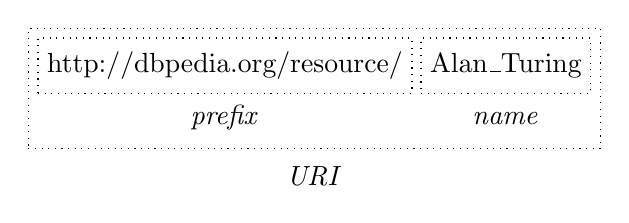
\begin{tikzpicture}[scale=1]
    \tikzstyle{part} = [draw,rectangle,dotted,fill=none,minimum height=0.7cm]
    %\tikzstyle{caption} = [plain,draw=none,fill=none]
    \tikzstyle{mylabel} = [text width=5em, text centered]
    \node[part] (prefix) at (0,0) {http://dbpedia.org/resource/};
    \node[part] (name) [right = 1mm of prefix] {Alan\_Turing};
    \node[mylabel] (label1) [below = 0.2mm of prefix] {\textit{prefix}};
    \node[mylabel] (label2) [below = 1.2mm of name] {\textit{name}};
    \node[part,fit=(prefix) (name) (label1) (label2)] (uri) {};
    \node[mylabel] (label3) [below = 1mm of uri] {\textit{URI}};
\end{tikzpicture}
  \caption{URI, prefix, name}
  \label{fig:uri-prefix-name}
\end{figure}

\noindent
Objects can be either URIs or literals, such as number, string or date. (Maybe TODO: priklady)
Simple example with prefixes (part of the graph above):

\begin{code}
<http://dbpedia.org/resource/Alan_Turing>
    <http://www.w3.org/1999/02/22-rdf-syntax-ns#type>
    <http://xmlns.com/foaf/0.1/Person> .
<http://dbpedia.org/resource/Alan_Turing>
    <http://dbpedia.org/ontology/birthDate>
    1912-06-23+02:00
<http://dbpedia.org/resource/Alan_Turing>
   <http://dbpedia.org/property/nationality>
   "British"@en
\end{code}

Besides this \textit{N-Triple} format
\cite[][68]{semantic-web}
there are several others serializations of RDF graph, such as \textit{RDF/XML}
\cite[][73]{semantic-web}
or \emph{Turtle (Terse RDF Triple Language)},
which makes the serialization shorter by grouping facts by subjects (and predicates) and by using shortcuts for prefixes. The same graph as above would look like this in the Turtle syntax:

\begin{code}
@prefix rsrc: <http://dbpedia.org/resource/>
@prefix rdf: <http://www.w3.org/1999/02/22-rdf-syntax-ns#>
@prefix dbpedia-owl: <http://dbpedia.org/ontology/>
@prefix dbprop: <http://dbpedia.org/property/>
@prefix foaf: <http://xmlns.com/foaf/0.1/>

rsrc:Alan_Turing
  rdf:type foaf:person ;
  dbpedia-owl:birthDate 1912-06-23+02:00 ;
  dbprop:nationality "British"@en .
\end{code}

RDF graphs are great for representation of simple facts, but it is useful to know about its limitaions. RDF graphs is designed to capture \textit{procedural knowledge}, such as mathematical problem solving,
[Maybe TODO: takze nemuzeme pak testovat higher order thinking skills... citace k tomu higher order thinking skills, napr. Bloom's taxonomy]


% ---------------------------  SECTION  ---------------------------
\section{SPARQL}
\label{sec:sparql}

\textit{SPARQL}%
\footnote{The name of this query language is a recursive acronym of \textit{SPARQL Protocol and RDF Query Language}.}
is a query language for convenient querying of RDF graphs. \parencite[][84]{semantic-web}.
The most common is the \textit{SELECT query} which resembles SQL SELECT query and has these main parts:
\begin{myItemize}
  \item \textbf{PREFIX} -- definition of prefixes and assosiated shortcuts,
  \item \textbf{FROM} -- dataset (RDF graph) on which to run the query,
  \item \textbf{SELECT} -- which information to return,
  \item \textbf{WHERE} -- condition on returned data,
  \item \textbf{ORDER BY} -- ordering of results.
\end{myItemize}
As an example, take a look at the following SPARQL query, which would return the birthdate and birthplace of Alan Turing:
\begin{code}
PREFIX rsrc: <http://dbpedia.org/resource/>
PREFIX owl: <http://dbpedia.org/ontology/>
SELECT ?date ?place
WHERE {
  rsrc:Alan_Turing owl:birthDate ?date ;
                   owl:birthPlace ?place .
}
\end{code}

%% ---------------------------  SECTION  ---------------------------
%\section{Ontology}
%\label{sec:ontology}

%TODO: ontologie - co to je, k cemu to je
%- v dalsi kapitole (odkaz) bude rozebrano, jak generovat otazky s vyuzitim ontologii

%O co jde: ontologií se rozumí popis vlastností, tříd a jejich hierarchie
%(mezi tridou a podtridou je "is-a" relationship)


% ---------------------------  SECTION  ---------------------------
\section{Named Entity Recognition}
\label{sec:terms-extraction}
\textit{Named entities}
are "information units like names, including person, organization and location names, and numeric expressions including time, date, money and percent expressions" \autocite{named-entity-recognition}.
Sometimes I will specifically refer to \textit{terms}, which are named entities other than numeric expressions.
Es an example, \textit{"Abraham Lincoln"} is a term, while \textit{"21 March 2015"} is a numeric expression
(and both are named entities).
The aim of the \textit{named entity recognion} is to discover all named entities in a text and and label them with their types. Common types of named entites are organization, person, location, date, time, money, percent, facility and geo-political entity \cite[][281]{nlp-python}. There are several approaches to the task of named entity recognition:
\begin{myItemize}
\item \textbf{Regular expressions}\\
  Regular expressions are especially good for numeric expressions as they typical follow reasonably simple rules.
  [Maybe TODO: nejake konkretni ukazky zjednodusenych regexu]
\item \textbf{List of terms}\\
  A simple way to find if some word or phrase is a named entity is to try to look it up in a list of named entities. There are for example publicly available \textit{gazetteers} -- lists of well-known geographical locations. However, this method is quite limited as it is impossible to have complete lists of all named entities.
(In particular there is infinitely many numeric expressions.)
Another problem is ambiguity of words, e.g. \textit{"Reading"} is a town in the United Kingdom, but not in the sentence \textit{"Reading is important for everyone's personal development."}
  [TODO: podobne lze pouzit i bazi znalosti ... a mozna Wordnet?]
  There is one exception when this method works great -- if there is a known list of terms which can appear in the text. For example for each article on the Wikipedia the list of terms can be built from internal links which appear in the article. I use this fact in the Smartoo (\autoref{sec:articles-parsing}).
\item \textbf{Frequency counting}\\
  After identifying nouns and noun phrases in the text, we count their frequencies and these which exceed some given threshold are considered as terms.
  This method is used for example in \cite{question-gen-mitkov}. It works reasonable well for terms recognition, but it can't discover numeric expressions.
This method can label as terms also common names which are frequently used.
A solution to this problem is to apply \textit{tf-idf weighting} which normalizes term frequency in the document by its frequency in all documents (or in common texts) \cite[][118]{information-retrieval}.
[Maybe TODO: citovat, kde se na NE recognition pouziva TF-IDF nebo neco podobneho]
\item \textbf{Machine learning}\\
  The most difficult, but also the most powerful method is to train a machine learning recognizer.
  [TODO: podrobneji, napr. \cite[][283]{nlp-python}, \autocite{named-entity-recognition}]
\end{myItemize}
Often, several of these approaches are combined (e.g. in \textit{The Mentor} they use regular experssions, gazetteers and a machine learning recognizer \cite{mentor}).

TODO: clanek "A survey of named entity recognition and classification" \autocite{named-entity-recognition}


% ---------------------------  SECTION  ---------------------------
\section{Relations Extraction}
\label{sec:relations-extraction}

TODO... nlp-knizka

TODO: \parencite{triples-acquisition}

TODO: dalsi clanky

TODO: + inspirace Procvicnikem-v1

% ---------------------------  SECTION  ---------------------------
\section{Knowledge Bases}
\label{sec:knowledge-bases}

There are several huge publicly available knowledge bases,
which try to capture as many facts about the world as possible.
Examples of popular knowledge bases are
\textit{DBpedia}\footnote{\url{http://dbpedia.org/}}
and \textit{Freebase}.\footnote{\url{https://www.freebase.com/}}
Knowledge bases are used for many task in natural lanuage processing,
such as named entity recognition [TODO: coz by se melo rozebirat v predhozi kapitole ?!],
desambiguation,
semantic search [Maybe TODO: co to znamena, citovat Google]
and question answering -- several knowledge bases (including DBpedia) were used in \emph{DeepQA project} to create \emph{IBM Watson} computer, which won the \emph{Jeopardy!} quiz game against two human champions in 2011 \cite{watson}. And we can make use of information in these knowledge bases to create better exercises as well. [TODO: upravit posledni vetu, zpresnit, kdy a k cemu budeme bazi znalosti vyuzivat]

DBpedia was built by extracting structured information from Wikipedia,
such as titles, links between articles, external links, information from infoboxes and categories.
Facts are stored in the form of an RDF graph.
Whole knowledge base can be be downloaded%
\footnote{\url{http://wiki.dbpedia.org/Downloads}, %
data available under \emph{Creative Commons Attribution-ShareAlike License}
and \emph{GNU Free Documentation License}}.
It also possible to use public \textit{DBpedia SPARQL endpoint}.%
\footnote{\url{http://dbpedia.org/sparql}}

\emph{DBpedia Version 2014}%
\footnote{\url{http://wiki.dbpedia.org/Downloads2014}}
contains approximately 580 million facts (RDF triples) retrieved from the English Wikipedia
describing 4.5 million of things \parencite{dbpedia}.
Ontology%
\footnote{Ontology is a description of properties, classes and their hierarchy.}
of DBpedia includes more than 650 classes and 2700 properties.
In \autoref{fig:dbpedia-classes} a fraction of DBpedia class hierarchy is shown.
\begin{figure}[h]
  \centering
  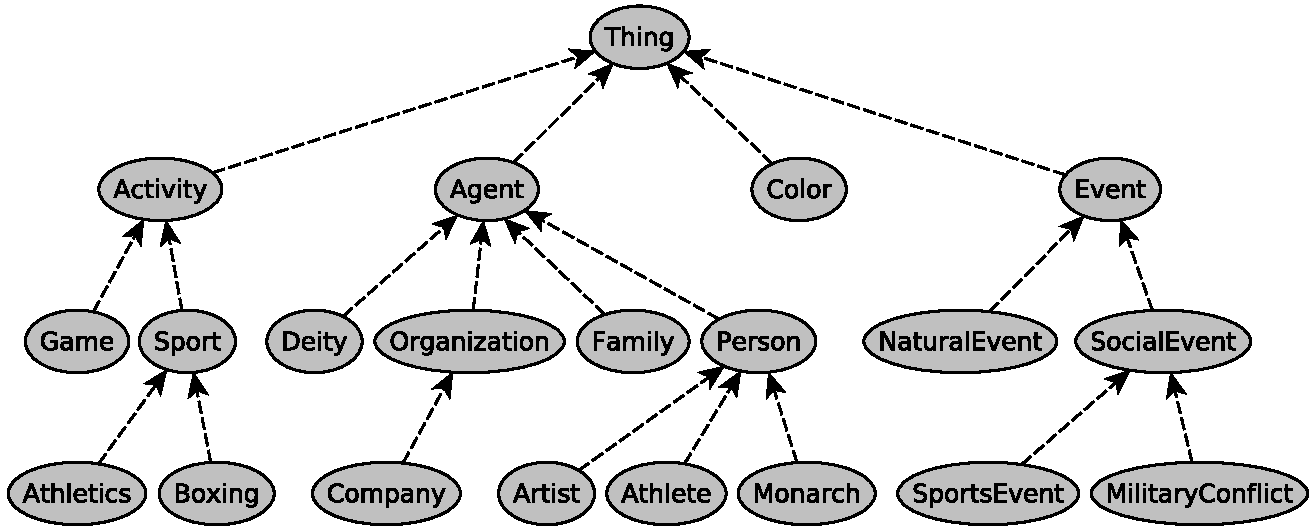
\includegraphics[width=\textwidth]{images/dbpedia-classes.pdf}
  \caption{A fraction of DBpedia class hierarchy. Edges represent subclass relationship.}
  \label{fig:dbpedia-classes}
\end{figure}

%\begin{verbatim}
%- Thing
%  - Activity
%    - Game
%    - Sport
%  - Agent
%    - Deity
%    - Family
%    - Organization
%    - Person
%      ...
%    ...
%\end{verbatim}

% ===========================  CHAPTER ===========================
\chapter{Question Generation}
\label{chap:exercises}

TODO: Obecny uvod, o co nam ted jde

Maybe TODO: da se zminit, ze je tezke pristupy navzajem porovnat, protoze jsou hodne ruznorode v cily (uceni ciziho jazyka, uceni se lingivistiky, reading comprehension, fakta z ucenbice biologie -- asi by to chtelo ocitovat), zdrojich a tedy ve vyhodnoceni; kazdopadne existuje nekolik asi pouzitelnych systemu, vzdy jsou ale zamysleny jako "ucitel nahraje text, system vyplivne radu otazek, ucitel je profiltruje a opravi pripadne chyby a pak ty otazky pouzije" ... vyhodnoceni casto formou, 2 lide (studenti lingvistiky/biologie) o kazde otazce reknou, jestli je ok, potrebuje upravy, nebo je totalne na nic... vybiraji ruzne pocty otazek (napr. 15 procent) - to taky samozrejme vyrazne ovlivnuje vysledek (ale tak zas mohli vybrat proste tak, aby byl vhodny pomer pokryti a presnosti, vetsi problem je asi v tom, ze je proste fittovane napr. na tu ucebnici biolobie)
Konkretne: ucebnice biologie \parencite{question-gen-textbooks}

Maybe TODO: snazime se tedy aspon systematizovat ruzne pristupy a identifikovat spolecne ukoly -- content selection, question formation, distractor selection, qustion grading and filtering


% ---------------------------  SECTION  ---------------------------
\section{Content Selection}
%\label{sec:}

First step in exercises generation is to decide what are we going to ask about, i.e. what content (knowledge) we want to test (or practice).
Ideally we would like to select the most important and relevant content, but it is not easy.
Some possible approaches to the content selection are listed and described below.

\begin{myItemize}
\item kazda veta, ze ktere lze vytvorit otazku
  (muzou byt i souveti), (nejake pravidlo, ktere vetu transformuje na otazku + odpoved, viz nasledujici sekce)

\item vyber vet podle relavance (machine learning)
pristup by Agarwal \parencite{question-gen-textbooks}:
1) nalezeni vet, ktere jsou dostatecne informativni a maji dostatek kontextu (features: frekvence tokenu z nadpisu, obsahuje zkratku, obsahuje superlativum, pocet slov, pocet podstatnych jmen, ...)\\
2) vyber klice (tj. kam se da mezera) (features: pocet vyskytu slova v dokumentu, zda je obsazene v nadpisu, hloubka v syntaktckem stromu dane vety)\\

\item vyber skupiny vet a z nich vytvorit otazku (aspon myslim, ze to nekde bylo.. jak bylo 6 otazek z jednoho odstavce???

\item z grafu znalosti  -- v nejjednodusim pripade 1 fakt (A -- narodil se -- 1970. Zeptame se na to, kdy se narodil A), ale lze i kombinovat (napr. mohli se potkat? vymyslet nekolik peknych prikladu)... umoznuje ptat se na otazky ktere spanuji cely text, odkaz na knowledge extraction, graf  a sparql a vzdy souvislost a ukazku - ano i ukazku dotazu!
\end{myItemize}

TODO: do tohoto kroku zaradit i vyber toho, na co se chceme zeptat (moznost popisovat uz v prubehu, napr. v grafu je to prirozene), jinakt to lze to delat ruzne (bude je to nektera pojmenovana entita - odkaz na named entities recognition, nebo pomoci strojoveho uceni (Argawal)


Maybe TODO: pristup s mezikrokem extrakce informaci (ale asi jen trochu, prozkoumat...): Heilman \cite{question-gen-heilman}


% ---------------------------  SECTION  ---------------------------
\section{Question Formation}
%\label{sec:}

Pote, co vybereme, na co se chceme zeptat, je potreba vytvorit vhodnou otazku, nebo obecneji cviceni na procviceni dane znalosti

There are many types of exercises, but we restrict our attention to the multiple choice questions as these are the most popular in automatic question generator tools.
\textit{Multiple choice questions} (MCQ) consists of a question text (called \textit{stem})
and a few (e.g. four) \textit{choices}, from which one is the \textit{correct answer}
and the rest are incoreect alternatives (called \textit{distractors}).
Special type of multiple choice question is \textit{fill-in-the-blank multiple choice question} (FMCQ),
in which the stem is simply sentence with a blank space to which the correct answer should be put [preformulovat].

Maybe TODO: MCQ -- ze jsou oblibene, maji sve vyhody a nevyhody, vyjmenovat

TODO: odkaz na priklad, nebo jeste lepe priklad rovnou uvest (muze to byt nejaky, na ktery se zpetne odkaze sem)

- souvisi s otazkou exercise type (MCQ) a question type (FMCQ), takze tady popsat ty pojmy


TODO: note -- zalezi, co je vystupem content selection -- veta, souveti, skupina vet, skupina faktu

- gap fill is easy, ale bezne typy otazek potrebuji vetne transformce.
- ty se daji zapsat pomoci nejakych pravidel z vet/faktu do vet - jak ziskat takova pravidla -- vetsina pristupu (citovat) rucne, nektere se snazi pouzit strojove uceni (bootstraping - the-mentor, citovat)


[Each sentence of given text (after parsing) is matched against patterns
and may produce question-answer pair.]

Approaches to stem generation can be divided according to how much they use the meaning (semantic information) (pro transformaci z vet, ale pro fakta z knowledge graphu by ty pristupy byly podobne):
\begin{myItemize}
\item \textbf{Syntactic approach}\\
  * z vety se tvori otazka, pokud obsahuje nejaky pojem a navic ma urcitou strukturu, napr.
    $$
    S V O \text{.} \longrightarrow \text{Which } H V O \text{?}
    $$
    where $S$, $V$, $O$ stand for \textit{subject}, \textit{verb} and \textit{object} and $H$ is the hypernym of the subject (found using WordNet). (TODO: uvest priklad)
  * TODO: dalsi priklady (i bez Wordnetu)
  * rozdelit a citovat pripady s harcoded rules vs. pravidla v externich sablonach
  * hardcoded transformation rules (overit):
    - Wolfe, 70. leta, \textit{AutoQuest} \cite{questions-wolfe};
    - Mitkov, 2006, \cite{question-gen-mitkov}:

  * i souveti (spojky): delal jsem taky neco podobneho loni (napr. X because Y), ze par prikladu a citace \cite{question-gen-connectives}, uvest priklad

  * from external templates: \textit{Ceist system} \cite{question-gen-ceist}

\item \textbf{Semantic approach}\\
  - od predchoziho pristupu se lisi v tom, ze transformacni pravidla pracuji se semantic role labels, napr. agent, patient etc;  cili (castecne) s vyznamem vety

  - Typy otazek popsane pomoci generickych sablon, ty popisuji vztah mezi vetou a otazkou (s vyuzitim sementickych roli a syntaktickych konstituentu, naprt. \texttt{What |verb| |patient| |location|?} with answer being \texttt{agent} atp., taky. specifikuji semanticou roli, kterou zastava odpoved atp.

  - Semanticky bez sablon: \cite{question-get-mannem}
  - semanticky se salonami: \cite{questions-eval}
\end{myItemize}

TODO: tohle bylo o vetach/souvetich, ale z faktu to bude fungovat podobne, akorat je to jeste trochu vid do semanticna (tj. jeste vice program pracuje s vyznamem textu), opet nejaky priklad pravidla, jak z faktu vytvorit text, mozna inspirace v Procvicniku loni

TODO: odstavec o tom, ze transformaci pravidla se tradicne psali rucne (at uz primo do programau, nebo pomoci externich sablon), ale v posledni dobe se ukazuje, ze je asi mozne tyto vzory naucit pomoci metod strojoveho uceni ....(system learns patterns in sentences which describe a relation between a question and an answer)  The approach of bootstrapping lexico-syntactic patterns was used
in \textit{The Mentor} system \cite{mentor}, created by Technical University of Lisbon.
(Boostrappping means ASI using only a few question-answer pairs as as seeds, new one are ?odvozene nebo co? [bootstrapped...]
... they are using \textit{QuestionBank} a corpus of 4000 parse-annotated questions \cite{question-bank}.
(no ten QuestionBank se pouziva jen na natrenovani syntaktickeho parseru)
[TODO: podrobneji, seed question-answr -> permutace moznosti, jak muze vypadat prislusna deklarativni veta -> jestli opravdu jo, se zjisti pomoci Googlu -> vytvoreni vzoru] [ale porad tam nechapu ten bootstrapping]




% ---------------------------  SECTION  ---------------------------
\section{Distractor selection}
\label{sec:distractors}

It is important to present a multiple-choice question with competitive \textit{distractors}.
As shown by experiments described in \cite{optimizing-multiple-choice}, multiple choice questions with competitive incorrect alternatives not only help to remember the correct answers to the original questions, but they also improve later performance on the previously nontested questions for which these alternatives may be the correct answers. If the alternatives are not competive, a student can recognize the correct answer without retrieval, just by pattern matching. As an example, consider the following multiple choice question:

\begin{exercise}
\caption{Question with noncompetitive alternatives}%\label{table:somename}
  \begin{question}
  Lincoln was assassinated by \sentenceGap , a Confederate sympathizer.
  \begin{choices}
    \choice Emancipation Proclamation
    \choice John Wilkes Booth
    \choice Illinois
    \choice Department of Agriculture
  \end{choices}
  \end{question}
\end{exercise}

Clearly, the student does not need to remember who assassinated Lincoln to answer this question correctly and they are also not forced to retrieve any knowledge about alternatives.
Of course, this was an extreme example to illustrate the point -- you definitely would not come accross such poor distractors in manually created multiple-choice questions.
Now take a look at the following question:

\begin{exercise}
\caption{Question with competitive alternatives}%\label{table:somename}
  \begin{question}
  Lincoln was assassinated by \sentenceGap , a Confederate sympathizer.
  \begin{choices}
    \choice Thomas N. Conrad
    \choice Robert E. Lee
    \choice John Wilkes Booth
    \choice Ward Hill Lamon
  \end{choices}
  \end{question}
\end{exercise}

This questions is much more likely to force student to retrieve knowledge about John Wilkes Booth as well as about other alternatives.

\cite{optimizing-multiple-choice} also showed that competitive distractors are not confused with correct answers in later questions more often than noncompetitive distractors.

The consequences are clear -- when creating a multiple-choice question, we should try to find plausible alternatives which are as competitive as possible.
A tak se skutecne deje v ruznych aktualnich systemech \cite{question-gen-mitkov, slepe-mapy}
NOTE: u systemu, kde je omezena fixni sada faktu k nauceni (slepe mapy), tak lze brat jako distraktory polozky, ktere se nejvice pletou (citovat slepe mapy). Common strategies for distractor selection are:
\begin{myItemize}
\item \textbf{Named entities from the text}\\
  One possibility is to use named entities from the text discovered by named entity recognition (\autoref{sec:terms-extraction}). As distractors, named entities of the same type are chosen (e.g. if the correct answer is person, choose people as distractors). This approach was used in the Mentor \cite{mentor} and OntoQue \cite{ontoque}.
If one term can have many types (which is the case in Smartoo), terms which has most types in common with the correct answer are selected.
As an alternative to common types, common context can be used to select appropriate distractors.
Agarwal \cite{question-gen-textbooks} uses features such as comparison of words and their POS tags before and after the correct answer and the distractor or frequency of common words in the question sentence and a sentence with the distractor.

\item \textbf{Named entities from external sources}\\
  Using \textit{WordNet} [citovat] or a knowledge base, we can find similar terms, even if they are not in the text. For example, in \cite{question-gen-mitkov} distractors for a term were found using \textit{coordination relation} in WordNet (coordinates are words sharing at least one hypernym). If more coordinates were found in WordNet, the ones which occur in the text are preffered.

\item \textbf{Correct answer modification}\\
  If the correct answer is a numerical expression, we can easily obtain distractors by changing the date or value by some partially random relative shift
\cite{question-gen-domain-ontologies}.
[TODO: priklad s letopoctem]
\end{myItemize}





% ---------------------------  SECTION  ---------------------------
\section{Question Ranking and Filtering}
%\label{sec:}

TODO: uvod, ze mnoho otazek bude of poor queality, nebo irelevantnich, co s tim: ohodnotit a vybrat N nejlepsich, nebo filtrovat (pravidlove, machine learning-based classifikator) (filtrovani je specialni druh hodnoceni, ktere je jen binarni)

Co citovat: vyber 6 nejlepsich otazek na odstavec \cite{question-gen-mannem}, filtrovani \cite{mentor}
(a i dalsi, filtrovani se objevilo casteji)


Maybe TODO: dokonce nejaky metody jsou vylozene zalozene na overgeneration a pak filtering (neco myslim bylo v te phd tezi, prip. v dalsich clancich od toho autora)


\cite{mentor}: Some filters are applied to discard questions of poor quality. Two main filters are:
\begin{enumerate}
  \item matching question-answer category:
    The category of the question and the category of the answer have to be same (e.g. individual or location). Example: "Who was Abraham Lincoln?" -- "16th president of the United States": both \textit{Abraham Lincoln} and \textit{president} has the semantic category \textit{individual}.
    To find that president is individual, WordNet [citovat] is used (BFS).
  \item Discarding Anaphoric References: e.g. "Where is there?"
\end{enumerate}

TODO: Prozkoumat clanek Question Generation via Overgenerating Transformations and Ranking, pro mozne zduvodneni komponenty ExercisesGrader, hodnoceni (pro vyber 6 nejlepsich otazek na odstavec) je take v
\cite{question-gen-mannem}

Maybe TODO: Muzu zde take rozebrat, jak jednotlive system vyhodnocovali


% ---------------------------  SECTION  ---------------------------
\section{Dalsi temata, todo}
\textbf{Generovani otazek s vyuzitim ontologii}

- generovani otazek s vyuzitim ontologii:
\cite{question-gen-domain-ontologies} -- popisuje ruzne strategie, jak z hotoveho grafu generovat otazky (coz je v nejjednodussim pripade proste vyber jednoho faktu) a k nim distraktory (i distraktory jen na urovni celych vet, zadani bylo vzdy "Choose the correct sentence"; priklady:
- pro RDF trojici A-B-C vytvor distraktor A-B-D, kde D je typu, ktery je podtridou typu C
- pro RDF trojici A-B-C, pokud je C numericka hodnota, vytvor distraktory jako nasobky (a podnasobky) dane hodnoty;

\textit{OntoQue} \cite{ontoque}, a system generating questions from a domain ontology.
Various question types: multiple choice questions, true/false, fill-in the blanks.
True/False: chybne vety jsou ze spravne vety vytvoreny nahrazenim subjektu nebo objektu za term, ktery je semanticky blizko (je ze stejne tridy).


..................

Maybe TODO: podivat se na "question generation workshops and the shared task (in 2010)"
http://questiongeneration.org/














% ===========================  CHAPTER ===========================
\chapter{Adaptive Practice}
\label{chap:practice}

TODO popis stavu: mame vygenerovane otazky (prip. i s ohodnocenim?), ted je chceme studentovi predkladat, v nasem settings: obvykle mame spousty otazek (destiky nebo stovky) ale predlozit jich ma cenu je nekolik (napr. 10 nebo 20, prip. dalsi na zadost uzivatele) ... je tedy dulezite umet vybrat ty nejvice pro studenta relevantni otazky a zaroven vyvazovat prumernou uspesnost (pokud by uzivatel nevedel nikdy spravnou odpoved, tak by ho to deprimovalo)

TODO: trochu jine podminky jsou, pokud jsou otazky (nebo aspon fakta) vytvoreny predem (napr. slepe mapy), ale i tam nas samozrejme zajima adaptabilni procvicovani a mnohe z nasledujiciho se vztahuje k obema pripadum

TODO o co jde: poskytovani tech otazek, ktere jsou pro uzivatele co nejuzitecnejsi ... tj. zamereni na to, co student jeste moc dobre neumi, ale na druhou stranu vyvazovat uspesnost (pokud by uzivatel nevedel na zadnou otazku spravnou odpoved, tak by ho to deprimovalo.

(TODO: mozne rozdeleni na 3 casti: odhad prior knowledge (nejspis na urovni jednoho faktu), odhad aktualni znalosti (ma smysl pri opakovanych otazkach na 1 fakt, napr. slepe mapy, ale nikoliv Smartoo), selection of a suitable question (podle odhadu znalosti a historie odpovedi).)


Takze napred projdu nekolik nejznamejsich zpusobu modelovani skillu studenta a obtiznosti faktu (IRT/Rash, PFA, ELO, PFAE, BKT), pak se zamerim na samotny vyber otazky.


% ---------------------------  SECTION  ---------------------------
\section{Item Response Theory}
\label{sec:irt}


TODO...

NOTE: Mozna zvlast sekce o IRT a Rash Modelu?

Napr. Rash Model, coz je logisticky model, predpoklad konstantni znalosti studenta (neuvazuje uceni). Pro multiple choice questions with $n$ options (tj. pravdepodobnost nahodneho uhadnuti je $\frac{1}{n}$), znalost studenta daneho faktu dana parametrem $s$ a obtiznost tematu dana parametrem $d$, vypada odhad spravne odpovedi nasledovne:

$$
P(correct \mid k, d) = \frac{1}{n} + \left( 1 - \frac{1}{n} \right) \cdot \frac{1}{1 + e^{-(s - d)}}
$$

(Mozne TODO: graf)

TODO: uceni parametru: joint maximum likelihood estimation (odkaz), offline, potreba dost dat a je to pomale a obzvlaste nevhodne pro online aplikace, kde je idealni kontinualni update


% ---------------------------  SECTION  ---------------------------
\section{Performance Factor Analysis}
\label{sec:pfa}

NOTE: Performance Factor Analysis = rozsireni Rash modelu, aby uvazoval meninic se znalost skillu; pravdepodbnost odpovedi je stale dana logaritmickou funkci, ale neni zavisla na konstantnim rozdilu znalosti studenta a obtiznosti faktu, ale na linearni kombinaci obtiznosti a poctu studentovych spravnych a poctu chybnych odpovedi na prislusnou otazku ($m = d + \alpha \cdot correctCount + \beta \cdot incorrectCount$).
Vsimneme si, ze v uvahu nebere poradi spravnych a spatnych odpovedi, pouze jejich obsolutni pocet (tj. neumi rozlisit mezi tim, ze jsem 10 krat odpovedel spatne a pak 10 krat dobre a mezi tim, ze odpovidam jednou dobre a jednou spatne.)

Dalsi problem je, ze nebere v uvahu moznost tipovani (coz je potreba u multiple choice otazek).

% ---------------------------  SECTION  ---------------------------
\section{Elo System}
\label{sec:elo}


TODO: inspirovane hodnocenim sachovych hracu \cite{elo-rating}, mozna i napred trochu popsat, jak to funguje tam a pak teprve ta analogie na nasi situaci

Je to dalsi zpusob, jak rozsirit Rash model o uceni, odhad spravne odpovedi zustava stejny logisticky model (odkaz na ten vzorecek). Skill se updatuje po "zapasu" mezi studentem a otazkou (faktem) nasledovne,
kde $s$ je skill studenta, $R$ je result (1 if the answer was correct, 0 if incorrect).
$$
s \gets s + K \cdot (R - P(R = 1))
$$

NOTE: Lze pouzit (a ve Slepych mapach \cite{slepe-mapy} se pouziva) i pro odhad prior knowledge (a global difficulty faktu)
(Oproti Rash modelu asi nema v tomto ohledu tak dobrou semantiku (viz clanek slepe-mapy), ale zato se lepe pocita, vhodny pro online system; navic experimenty ukazuji, ze se to chova podobne (odkaz opet v clanku ve slepe-mapy).
Pak je ale problem with constant K: kdyz je moc mala, tak je uceni pomale, kdyz je velke, tak nestabilni, je tedy vhodne (a pouziva se v Slepe mapy -- viz \cite{slepe-mapy}, mozna odkaz spis primo na system) pouzit misto konstanty
uncertainty function, e.g. $K = \frac{a}{1 + bn}$, kde $n$ je kolik otazek uz uzivatel zodpovedel (nebo obracene, kolik otazek na dane misto jiz bylo zodpovezeno) a $a$ a $b$ jsou fixne zvolene parametry.

Moznost zkombinovat PFA a Elo (viz \cite{slepe-mapy}, nazyvaji to PFAE, kde E muze znamenat bude Elo nebo Extended), porad stejna logisticka funkce, nyni vzhledem k $K_{sf}$, coz je odhad, ze student $s$ zna fakt $f$. Tato promenna (odhad) se updatuje po kazde otazce studenta $s$ na otazku na fakt $f$ podle vzorce pro Elo (odkaz), akort misto jedne konstanty $K$ se pouzivaji 2 ruzne pri spravne vs. spatne odpovedi.


% ---------------------------  SECTION  ---------------------------
\section{Bayesian Knowledge Tracing}
\label{sec:bayesian-network}

TODO: Baysovska sit (HMM) k popisu konceptu (skill) a jejich nauceni (2 stavy: known (learned) and unknown (unlearned)), 4 parametry modelu: pravdepodobnost, ze je koncept known hned od zacatku, pravdepodobnost nauceni v 1 kroku, pravdepodobnost spravne odpovedi, kdyz koncept neumim (guess) a pravdepodobnost spatne odpovedi, kdyz koncept umim (slip).
Update skillu po odpovedi na otazku: s pouzitim Bayesova pravidla.
Odhad parametru: napr. pomoci Expectation Maximization na existujicich datech.

Predpoklad je diskretni prechod z neumim do umim (coz je obvykle dost zjednodusujici, zapamatovani deklarativnich faktu je postupne).

Priklad systemu pro uceni, ktery vyuziva BKT: \cite{question-gen-adapt-bayes} (trochu rozebrany nize).

TODO: Dalsi clanky viz odkazy v clanku slepe-mapy.


% ---------------------------  SECTION  ---------------------------
\section{Question Selection}
\label{sec:question-selection}

NOTE: predchozi sekce (mozna to mely byt jen podsekce, ale to je jedno) se zabyvaji, tim, jak modelovat znalost studenta a obtiznost konceptu/faktu. To je jedna z komponent, kterou pro vyber vhodne otazky potrebujeme.

Kriteria, ktera jsou dulezita pro vyber vhodne otazky:

\begin{myItemize}
  \item relevance -- obecne relevance pro studenta, v nasem kontextu hlavne relevance k danemu tematu, v jinem to muze znamenat vice aktualni relevanci - co zrovna ted potrebuje student procvicit nejvice (least known concept -- napr. \cite{question-gen-adapt-bayes} ... neni potreba uplne resit pokud cekam, ze tam bude uzivatel dost dlouho a casem se dostnane ke vsemu)
  \item difficulty -- pro testovani je nejvhodnejsi, pokud je pravdepodobnost spravne odpovedi 50 procent (takova otazka pak poskytuje nejvice informaci o studentovych znalostech), ale pro procvicovani je je 50 procent uz dost malo a pusobi spise deprimacne, takze je dobre mirit vyse (napr. ve slepych mapach je 75 procent, zase by se hodil nejaky odkaz), rozhodne ne zas moc lehke, je to potreba vybalancovat (flow).
  \item variability -- to muze v ruznych kontextech znamenat ruzne veci, napr. stridat typy otazek, nebo neptat se na jeden pojem 2 krat za sebou (i kdyz jinou otazkou)
\end{myItemize}

Casty pristup je takovyto: tato (pripadne i nejaka dalsi) kriteria se pak mohou podili nejakou vahou na skore otazky, vybrana je pak otazka s nejvyssim skore (napr. slepe mapy -- citovat)

Dalsi takovy system je
\cite{question-gen-adapt-bayes}, vyuziva BKT pro modelovani studentovych znalosti a obtiznosti konceptu,  domenove nezavisle, vyber tematu otazky: least known concept, vyber konkretni otazky: bere se v uvahu primerena obtiznost a pestrost typu otazek.




% ===========================  CHAPTER ===========================
\chapter{Smartoo Framework}
\label{chap:smartoo}

TODO: obecny uvod, framework x prototype (deployed), modularita (zduraznit) - decomposition into the following components:
\begin{myItemize}
\item \textbf{KnowledgeBuilder} -- takes an article as the input and builds knowledge graph -- RDF graph of facts contained in the article.
\item \textbf{ExercisesCreator} -- creates a set of questions (or other types of exercises) using the built knowledge graph.
\item \textbf{ExercisesGrader} -- evaluates exercises with respect to attributes such as difficulty or relevance to the original article.
\item \textbf{Practicer} -- controls the practice session itself, i.e. gives the student one exercise at a time based on previous exercises and answers.
\end{myItemize}
Each component (e.g. \textit{KnowledgeBuilder}) has variable behavior (e.g. \textit{KnowledgeBuilderBehavior}), which is a parametrised code, i.e. an implementation of the behavior (the code) and a set of parameters which the code uses.
Component itself is just a wrapper around the behavior which performs common tasks, most importantly persistence management.
%(For example \textit{KnowledgeBuilder} stores the knowledge graph built byt its behavior.)
At the beginning of a new session, random 4-tuple of components with behaviors is chosen.%
\footnote{The selection is not actualy completely random, behaviors with better performance in the past are preferred over the behaviors with worse performance, see section \autoref{sec:smartoo-behaviors-selection} for details.} The described relationships are visualized in \autoref{fig:smartoo-architecture}.


\begin{figure}[h]
  \centering
  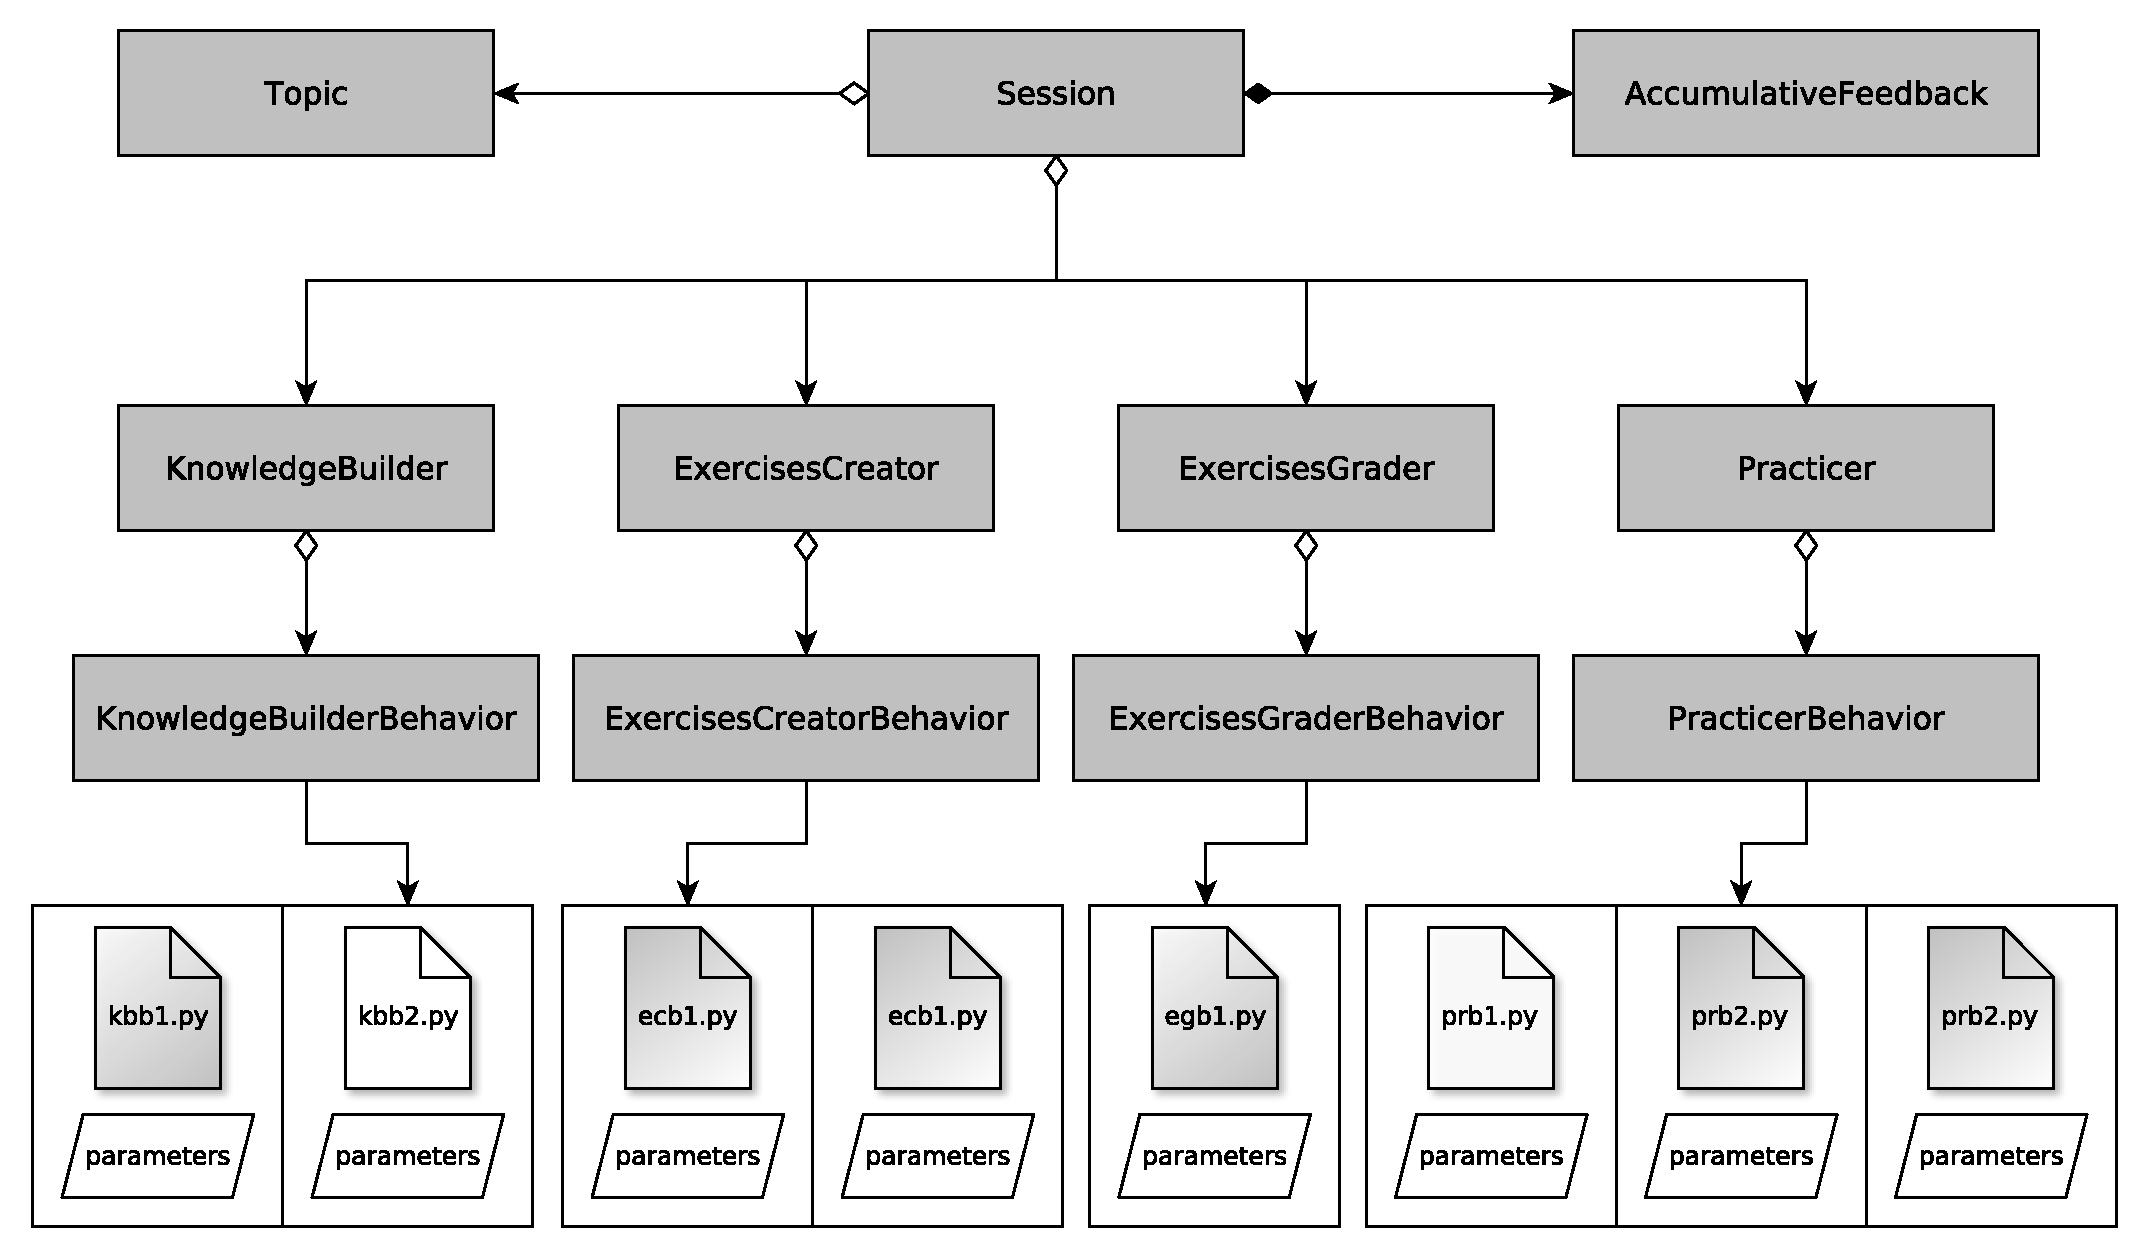
\includegraphics[width=\textwidth]{images/architecture.pdf}
  \caption{Components and behaviors}
  \label{fig:smartoo-architecture}
\end{figure}

Except from \textit{ExercisesCreator} and \textit{ExercisesGrader}
the components does not communicate with each other directly,
but via results (knowledge graphs and exercises) stored in the database.
The communication and the flow of data is depicted in \autoref{fig:data-flow-diagram}.
Individual processes are triggered by signals from client.
Time ordering of the signals and processes is showed in \autoref{fig:client-server-communication}.

\begin{figure}[h]
  \centering
  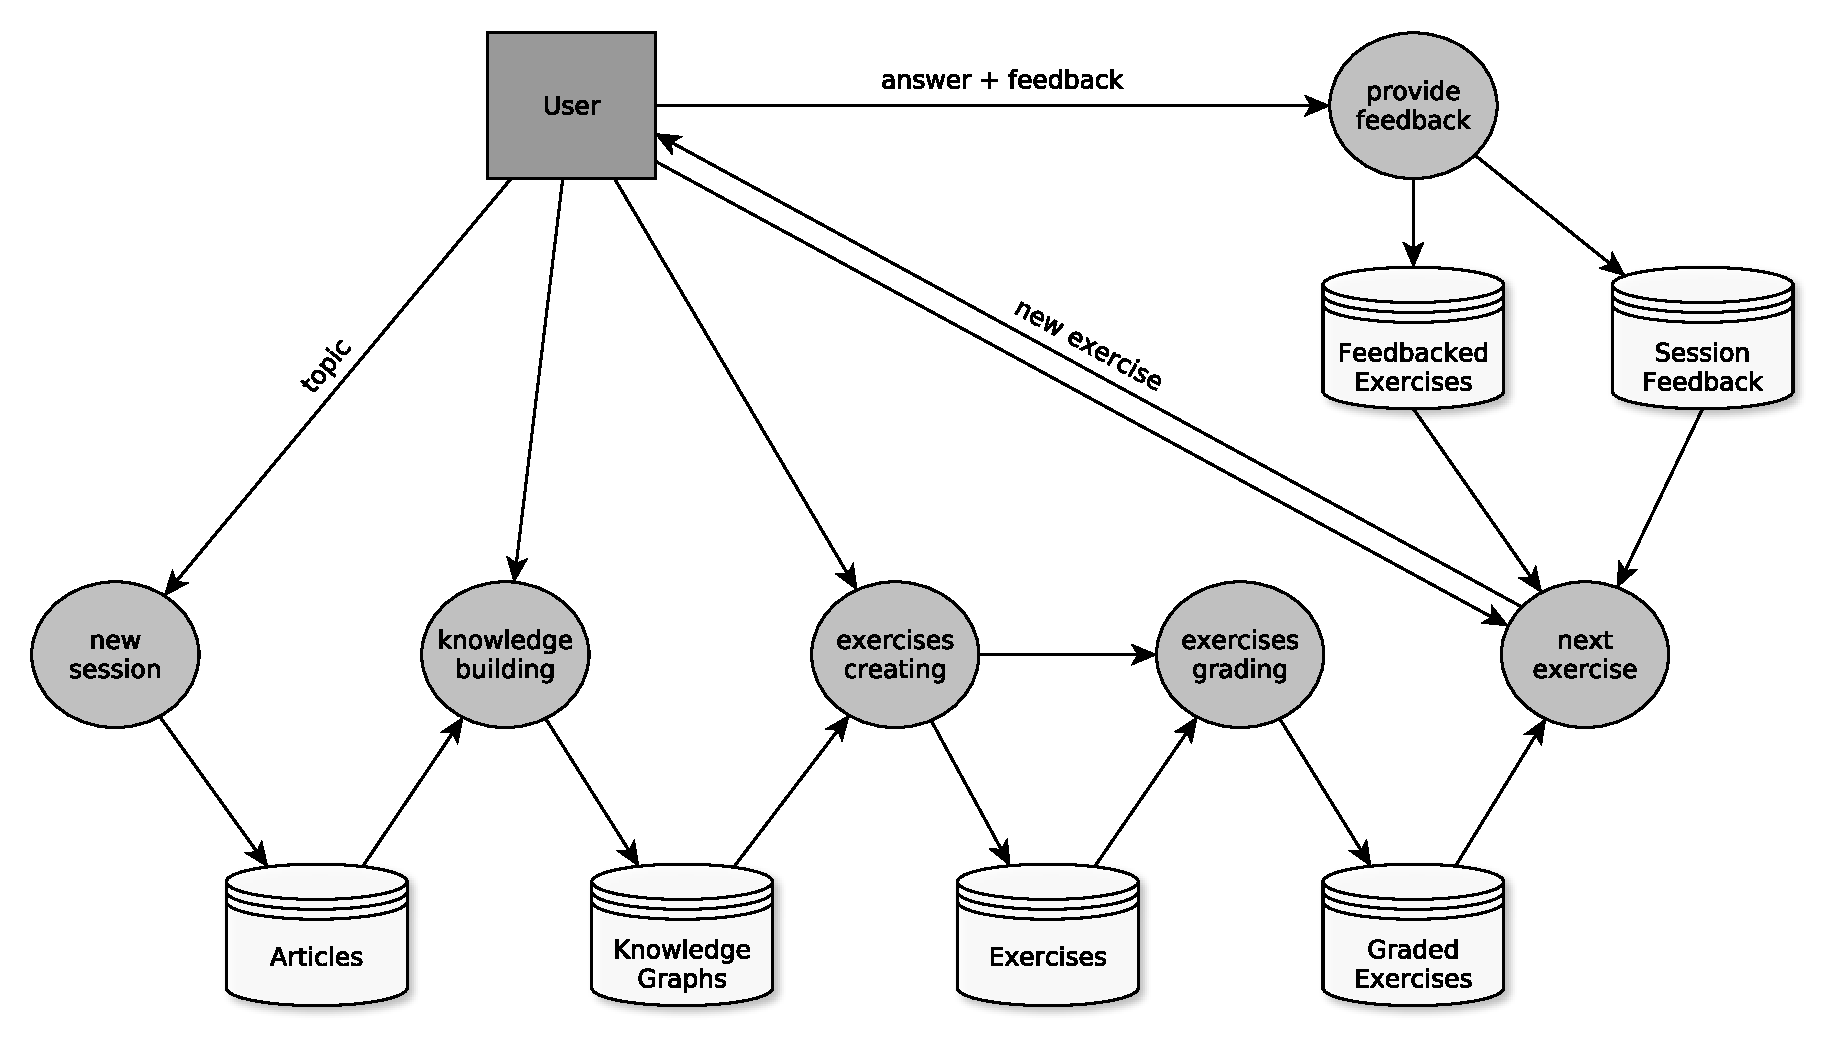
\includegraphics[width=\textwidth]{images/data-flow-diagram.pdf}
  \caption{Data flow diagram}
  \label{fig:data-flow-diagram}
\end{figure}

% ---------------------------  SECTION  ---------------------------
\section{Behaviors selection}
\label{sec:smartoo-behaviors-selection}

Each session has assigned a \textit{performance} which is computed as a weighted sum of the user final rating and the number of exercises marked as invalid or irrelevant. [Maybe TODO: presny vzorec]
As we know which behaviors participated in each session, we can compute the average performance of a 4-tuple of behaviors $p(x_1, x_2, x_3, x_4)$.

At the beginning of each new session, 4-tuple of behaviors $(k_1, k_2, k_3, k_4)$ ($k_1$ is knowledge builder, $k_2$ exercises creator, etc.) is chosen in a partially random way
which prioritizes behaviors with better performance in the past.
Ideally, the probability of a certain 4-tuple being selected would be proportional to its expected relative performance
(relative with respect to the expected performance of other 4-tuples).
As we do not know the future, our best guess for expected performance is the performance in the past.
Using conditional probability we can easily derive formulae for probability $P$ of components $(x_1, x_2, x_3, x_4)$ being selected.
I use asterisk ($*$) to denote "any behavior", so e.g. $p((x_1, *, *, *))$ means average performance of all sessions in which knowledge builder was $x_1$.
$$
P(k_1 = x_1) = p((x_1, *, *, *)),
$$
$$
P(k_2 = x_2 \mid k_1 = x_1)
  = \frac{P(k_1 = x_1 \land k_2 = x_2)}{P(k_1 = x_1)}
  = \frac{p((x_1, x_2, *, *))}{p((x_1, *, *, *))},
$$
$$
P(k_3 = x_3 \mid k_1 = x_1 \land k_2 = x_2)
  = \frac{P(k_1 = x_1 \land k_2 = x_2 \land k_3 = x_3)}{P(k_1 = x_1 \land k_2 = x_2)}
  = \frac{p((x_1, x_2, x_3, *))}{p((x_1, x_2, *, *))},
$$
and similarly for the fourth component.



TODO: Rozepsat a odargumentovat poradneji. (Bayes...)


% ---------------------------  SECTION  ---------------------------
\section{Articles Parsing}
\label{sec:articles-parsing}

If the user requests topic which were never requested before,
the corresponding article is looked up and retrieved from Wikipedia.
Some text preprocessing is performed, e.g. sections without useful content, such as "See also", "External links" or "References", are discarded.
Then the article is parsed into sentence trees with marked terms occurences.

\subsection*{Shallow Parsing}
Text is split into sentences and each sentence is tokenized (tokens are words, but also puctuation).
    Each token is assigned \textit{part-of-speech tag}.
    Part-of-speech tag denotes lexical category (also known as word class) of the word, such as noun, verb, adjective or determiner.
    For these natural language processing tasks I have used the \textit{NLTK} (Natural Language Toolkit) library \cite{nlp-python}. NLTK uses \textit{The University of Pennsylvania (Penn) Treebank Tag-set} \cite{penn-tagset}.

\begin{table}[h]
\begin{center}
\begin{tabular}{| l | l | l |}
  \hline
  Tag & Description & Example \\
  \hline \hline
  NN & common noun, singular & house         \\ \hline
  NNP & proper noun, singular & Lincoln     \\ \hline
  DT & determiner & the \\ \hline
  VB & verb, base form & eat \\ \hline
  JJ & adjective & popular \\ \hline
\end{tabular}
\end{center}
\caption{Part-of-speech tags examples \cite{penn-tagset} }
\end{table}

As an example, consider sentence \textit{"Six days after the surrender of Confederate commaning general Robert E. Lee, Lincoln was assassinated byt John Wilkes Booth, a Confederate sympathizer."} This sentence would be tokenized and tagged as follows:
\begin{code}
[['Six', 'CD'], ['days', 'NNS'], ['after', 'IN'], ['the', 'DT'],
['surrender', 'NN'], ['of', 'IN'], ['Confederate', 'NNP'],
['commanding', 'NN'], ['general', 'NN'], ['Robert', 'NNP'],
['E.', 'NNP'], ['Lee', 'NNP'], [',', ','], ['Lincoln', 'NNP'],
['was', 'VBD'], ['assassinated', 'VBN'], ['by', 'IN'],
['John', 'NNP'], ['Wilkes', 'NNP'], ['Booth', 'NNP'],
[',', ','], ['a', 'DT'], ['Confederate', 'NNP'],
['sympathizer', 'NN'], ['.', '.']],
\end{code}

\subsection*{Terms Occurences Inference}
In addition to text of the article, I also retrieve lists of titles of \textit{internal links}, i.e. links to another page on the Wikipedia.
These link titles can be thought of as a terms (as they have their page on the Wikipedia).
This terms are shallowed-parsed (tokenized and tagged)
and then I try to infer their occurences in the text.
In order to make the inference fast (meaning time complexity of $\mathcal{O}(n)$, where $n$ is the number of tokens in text), I first build a trie [TODO: vysvetlit nebo aspon odkaz] from all terms and then make a single pass through the text searching for longest matching terms in the trie. [TODO: urcite jde o nejaky znamy algoritmus nad retezci (nebo jeho variaci), pak by bylo fajn zminit jeho jmeno]
[TODO: uvest odkaz nebo odargumentovat casovou slozitost: sestaveni trie: celkovy soucet tokenu termu < delka textu, pak staci jediny pruchod textem]

%Stored content of an article looks like this:
%\begin{code}
%{'terms': [
%    ['Abraham Lincoln', [['Abraham', 'NNP'], ['Lincoln', 'NNP']]],
%    ['Robert E. Lee', [['Robert', 'NNP'], ['E.', 'NNP'], ['Lee', 'NNP']]],
%    ... ],
%'sentences': [ ...,
%    [['Six', 'CD'], ['days', 'NNS'], ['after', 'IN'], ['the', 'DT'],
%     ['surrender', 'NN'], ['of', 'IN'], ['Confederate', 'NNP'],
%     ['commanding', 'NN'], ['general', 'NN'], ['Robert', 'NNP'],
%     ['E.', 'NNP'], ['Lee', 'NNP'], [',', ','], ['Lincoln', 'NNP'],
%     ['was', 'VBD'], ['assassinated', 'VBN'], ['by', 'IN'],
%     ['John', 'NNP'], ['Wilkes', 'NNP'], ['Booth', 'NNP'],
%     [',', ','], ['a', 'DT'], ['Confederate', 'NNP'],
%     ['sympathizer', 'NN'], ['.', '.']],
%    ... ]
%}
%\end{code}

[Maybe TODO: terms inference podrobneji (a diagram)]

To represent shallowed parsed sentces with marked terms occurences,
I use shallow sentence trees.
You can see an example of a sentence tree in \autoref{fig:sentence-tree}.

\begin{figure}[h]
  \centering
  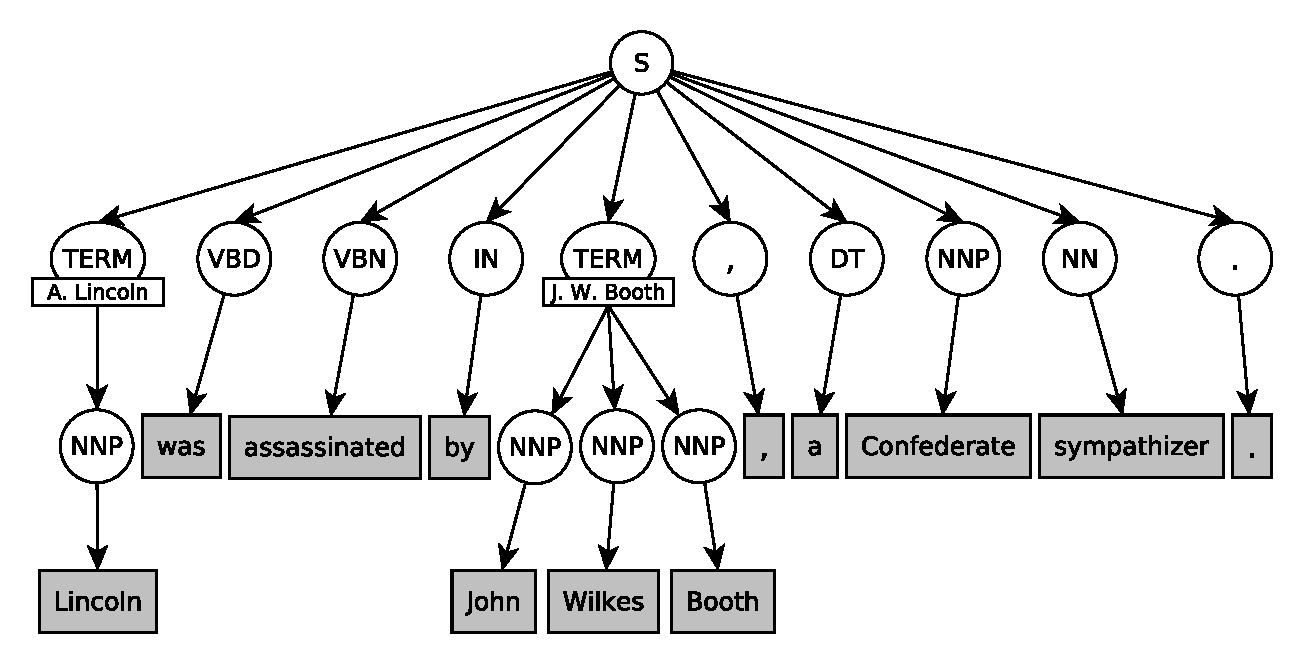
\includegraphics[width=\textwidth]{images/sentence-tree.pdf}
  \caption{Sentence tree}
  \label{fig:sentence-tree}
\end{figure}

% ---------------------------  SECTION  ---------------------------
\section{Knowledge Building}
\label{sec:smartoo-knowledge}

\textit{KnowledgeBuilder} component is responsible for building knowledge graph from given article.
Knowledge graph is RDF graph of facts contained in the article.

%\subsection*{Prototype Behavior}

Prototype behavior creates graph of \textit{quasi facts} about terms in sentences.
By the term \textit{quasi fact} I mean some information usable for creating exercises, but not really an elementary unit of knowledge, which ordinary facts should be. The algorithm is simple:
\begin{myEnumerate}
  \item Firstly, an empty graph is created (let us call it $G$).
  \item If it was not already in the past, knowledge graph of the topic term is retrieved from DBpedia (\autoref{sec:knowledge-bases}). All terms in this retrieved knowledge graph and also all terms in the article are added into the graph $G$ together with their types and labels (which are also found using DBpedia).
  \item Then we take each sentence in the article and check if it contains a term and is understandable without a context. The used heurisic is: it contains between 5 and 35 tokens (or 50, depending on the selected parameters), does not contain pronouns, parentheses or quotations or some typical anaphoric words (reffering to the context) such as "this".
  \item For each setence which satisfies these conditions, we create an quasi fact about the term in this sentence (and add it to $G$). Each quasi fact consists of several pieces of information: text before the term, text after the term and the term itself (and its label and types). An example of a created quasi fact can be seen in \autoref{fig:quasi-fact}.
  \item Graph $G$ is returned.
\end{myEnumerate}


\begin{figure}[h]
  \centering
  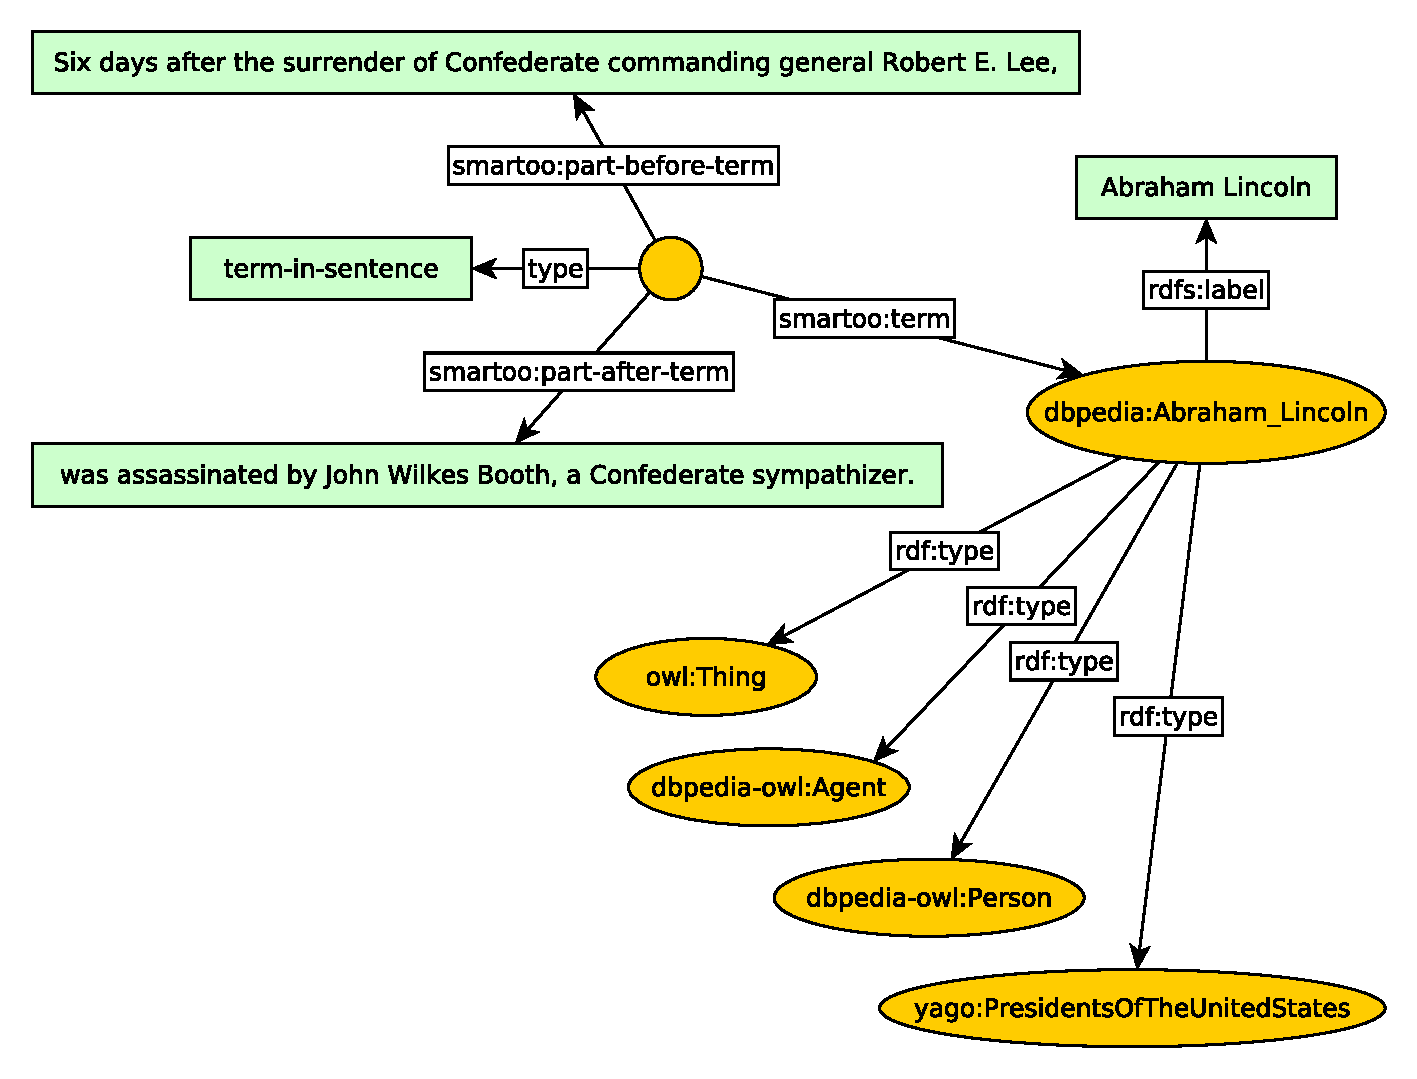
\includegraphics[width=\textwidth]{images/quasi-fact-lincoln.pdf}
  \caption{Example of a quasi-fact}
  \label{fig:quasi-fact}
\end{figure}

% ---------------------------  SECTION  ---------------------------
\section{Exercises Creating}
\label{sec:smartoo-exercises}

\textit{ExerciseCreator} component uses built knowledge graph to generate a set of exercises.
Exercises consists of presentaion data and semantic information.
\begin{myItemize}
  \item \textbf{presentation data}\\
    Currently the only supported type of exercise is a multiple choice question. Presentation data for multple choice question consists of the a question string, a list of choices labels and a correct answer label (which must be one of the choices labels).
  \item \textbf{semantic information}\\
    Semantic information is used for exercises graders. For this purpose I decided to use a list of term pairs for which holds, that if the user confuses them, it can lead to an incorrect answer.
    For a multiple choice question which correct answer $A$ and distractors $B$, $C$ and $D$,
    the semantic pairs are $(A, B)$, $(A, C)$ and $(A, D)$.
\end{myItemize}


Protype behavior uses all the quasi facts about terms in a sentence and creates "fill in the gap" questions with multiple options.
All quasi facts about terms in sentence can be retrieved from the knowledge graph with the following simple SPARQL query:
\begin{code}
SELECT ?before ?term ?after
WHERE {
    ?quasifact a "term-in-sentence" .
    ?quasifact smartoo:part-before-term ?before .
    ?quasifact smartoo:part-after-term ?after .
    ?quasifact smartoo:term ?term .
}
\end{code}

As we have multple choice question, we also need to select appropriate distractors.
Guided by the results about distractors presented in \autoref{sec:distractors},
the most similar terms to the correct answer are chosen.
Terms similarity heuristics is based on the number of common types
$C(t_1, t_2) = |types(t_1) \cap types(t_2)|$:
$$
sim(t_1, t_2) = 2 \left( \frac{1}{1 + \exp({-|C(t_1, t_2)| / \kappa})} \right) - 1
$$
The constants $\kappa$ influences the speed of convergence to $1$.
Terms without any common type would have $0$ similarity and the more common types they have, the more close to $1$ the similarity is. [Maybe TODO: 2 konkretni priklady podle poctu spolecnych typu, graf teto funkce v zavislosti na poctu spolecnych typu]

As an example, let us look at the exercise created from the quasi fact in \autoref{fig:quasi-fact}. The presentation data looks like this:
\begin{code}
{'question': 'Six days after the surrender of Confederate commanding
              general Robert E. Lee, _______ was assassinated by
              John Wilkes Booth, a Confederate sympathizer.',
'choices': ['Andrew Johnson', 'James Buchanan',
            'Abraham Lincoln', 'Franklin D. Roosevelt'],
'correct-answer': 'Abraham Lincoln'}
\end{code}
It corresponds to the following presentation of the exercise:
\begin{exercise}
\label{exrc:assassination}
\caption{Example of a created question}
  \begin{question}
  Six days after the surrender of Confederate commanding general Robert E. Lee
  \sentenceGap
  was assassinated by John Wilkes Booth, a Confederate sympathizer.

  \begin{choices}
    \choice Andrew Johnson
    \choice James Buchanan
    \choice Abraham Lincoln
    \choice Franklin D. Roosevelt
  \end{choices}
  \end{question}
\end{exercise}

And the respective semantic information is following:
\begin{code}
{'term-pairs': [
    ['Abraham Lincoln', 'Franklin D. Roosevelt'],
    ['Abraham Lincoln', 'James Buchanan'],
    ['Abraham Lincoln', 'Andrew Johnson']]}
\end{code}

% ---------------------------  SECTION  ---------------------------
\section{Exercises Grading}
\label{sec:smartoo-exercises-grading}

\textit{ExerciseGrader} takes an exercise (in particular the semantic part) and assigns it grades for difficulty, relevance to the article and possibly any other attributes, e.g. syntactic and grammatical correctness probability. All grades are numbers between $0$ and $1$. For the relevance, $1$ means the most relevant, for the difficulty $1$ means the most difficult.

In prototype behavior, grading is done via simple heuristics.
Difficulty of an exercise is estimated as the average similarity between all term pairs which can be mistaken.
Similarity of two terms is measured in the same way as in exercise creating (\autoref{sec:smartoo-exercises}).
[Maybe TODO: priklad paru u nejake otazky] [Maybe TODO: pro bylo zvoleno, vlastnosti, vyhody, nevyhody]

Relevance of the exercise is estimated as the \textit{cosine similarity} meassure between the exercise and the article,
i.e. cosine of an angle between the article and the exercise represented as sparse vectors mapping terms to their frequency in the article or the exercise
\cite[][121]{information-retrieval}.
Cosine similarity between two documents (in our case one document is the article $A$ and another is the exercise $E$) is given by the following formula:
$$
similarity(A, E)
= \frac{A \cdot E}{|A| |E|}
= \frac{\sum_{i=1}^{n} A_i E_i}{\sqrt{\sum_{i=1}^{n} A_i^2}\sqrt{\sum_{i=1}^{n} E_i^2}}
$$
where $A_i$ ($E_i$) denotes numbers of occurences of the $i$-th term in article (exercise).
This measure is commonly used in the information retrieval for estimating similarity between two documents of arbitrary length. The cosine similarity is a real number between $0$ and $1$, the higher it is, the smaller is the angle between documents in the vector space and the more similar the documents are. [Maybe TODO: obrazek s grafickym znazornenim onoho uhlu mezi article a exercise]


\section{Adaptive Practice}
\label{sec:smartoo-practice}

Task of the \textit{Practicer} is to control the practice session itself, i.e. to give the student one exercise at a time based on previous exercises and answers.

Prototype behavior of adaptive practicer is a .... [TODO: jak modeluje studenta... spis nijak, proste se snazim cilit na pozadovanou pravdepodobnost uspechu / simple heuristic...]
To select the most suitable exercise, three attributes of exercises are considered:
\begin{myItemize}
  \item relevance to the article,
  \item difficulty (compared to the so far success of the user),
  \item repetitiveness (to not ask about one term over and over again).
\end{myItemize}
Weights of these three attributes as well as the target success
are given by the behavior parameters.
\begin{table}[h]
\begin{center}
\begin{tabular}{| l | c | r | r |  r  |  r |  r | r |}
  \hline
  parameter & symbol & \multicolumn{6}{|c|}{used values} \\
  \hline \hline
  target success & $\tau$          & $0.75$ & $0.75$ & $0.75$ & $0.75$ & $0.75$ & $0.75$\\ \hline
  relevance weight & $\alpha$      & $1.00$ & $1.25$ & $1.00$ & $1.00$ & $1.25$ & $1.25$\\ \hline
  difficulty weight & $\beta$      & $1.00$ & $1.00$ & $1.25$ & $1.00$ & $1.00$ & $1.25$\\ \hline
  repetitiveness weight & $\gamma$ & $0.30$ & $0.30$ & $0.30$ & $0.60$ & $0.60$ & $0.60$\\ \hline
\end{tabular}
\end{center}
\caption{Parameters of prototype adaptive practice behavior}
\end{table}

\begin{myItemize}
  \item Relevance of the exercise was computed by \textit{ExercisesGrader}
(\autoref{sec:smartoo-exercises-grading}).

  \item Difficulty penalization is based on the difference between the target difficulty and the exercise difficulty.
Target difficulty is not exactly $(1 - \tau)$ as it is adjusted according to
so far success of the user -- if the correct ratio of the user is higher than the target success,
the target difficulty is set higher than $(1 - \tau)$ and vice versa.
(TODO: odkaz na experimenty na slepych mapach, kde se tohle ukazalo jako uzitecne)
(TODO: konkretni vzorec podle zdrojaku)

  \item Repetitiveness penalization is based on the cosine similarity between the scored exercise and the exercises already used in the current session
(see \autoref{sec:smartoo-exercises-grading} for the explanation and formula of the cosine similarity).
\end{myItemize}
The total score is given as weighted sum of the three individual scores described above.
$$
\text{totalScore} = \alpha \cdot \text{relevanceScore} + \beta \cdot \text{difficultyPenalty} + \gamma \cdot \text{repetitivenessPenalty}
$$
An exercise with the highest score is chosen.

TODO: priklad 1 session, otazek a odpovidani na, aby bylo videt prizpusobovani -- takze mozna jen pomoci nejakeho grafu s vyznacenymi dobrymi a spatnymi odpovedmi a aktualni target difficulty.


% ---------------------------  SECTION  ---------------------------
\section{Web Interface}
\label{sec:smartoo-web}

I have created a simple web interface for Smartoo,
using \textit{Boostrap}%
\footnote{\url{http://getbootstrap.com/}},
HTML and CSS framework for responsive design,
and {\textit{AngularJS}%
\footnote{\url{https://angularjs.org/}},
JavaScript framework for \textit{MVC} (Model -- View -- Controller) design%
\footnote{Actually, AngularJS states it is \textit{MVW} (Model -- View -- Whatever) framework, as it supports more aprroaches than just MVC.}.

\begin{figure}[h]
  \centering
  
\includegraphics[width=0.9\textwidth]{images/home-page.png}
  \caption{Smartoo home page}
  \label{fig:smartoo-home}
\end{figure}

\begin{figure}[h]
  \centering
  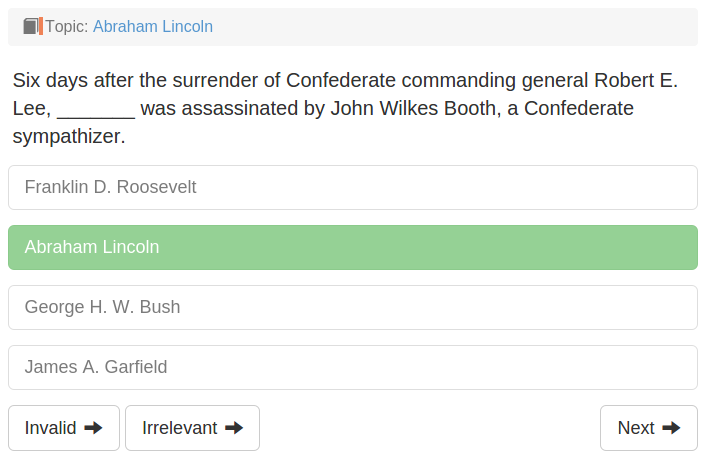
\includegraphics[width=0.9\textwidth]{images/answered-correctly.png}
  \caption{Correctly answered question}
  \label{fig:correctly-answered-question}
\end{figure}

The typical sequence of client requests and server responses is shown in
\autoref{fig:client-server-communication}

\begin{figure}[h]
  \centering
  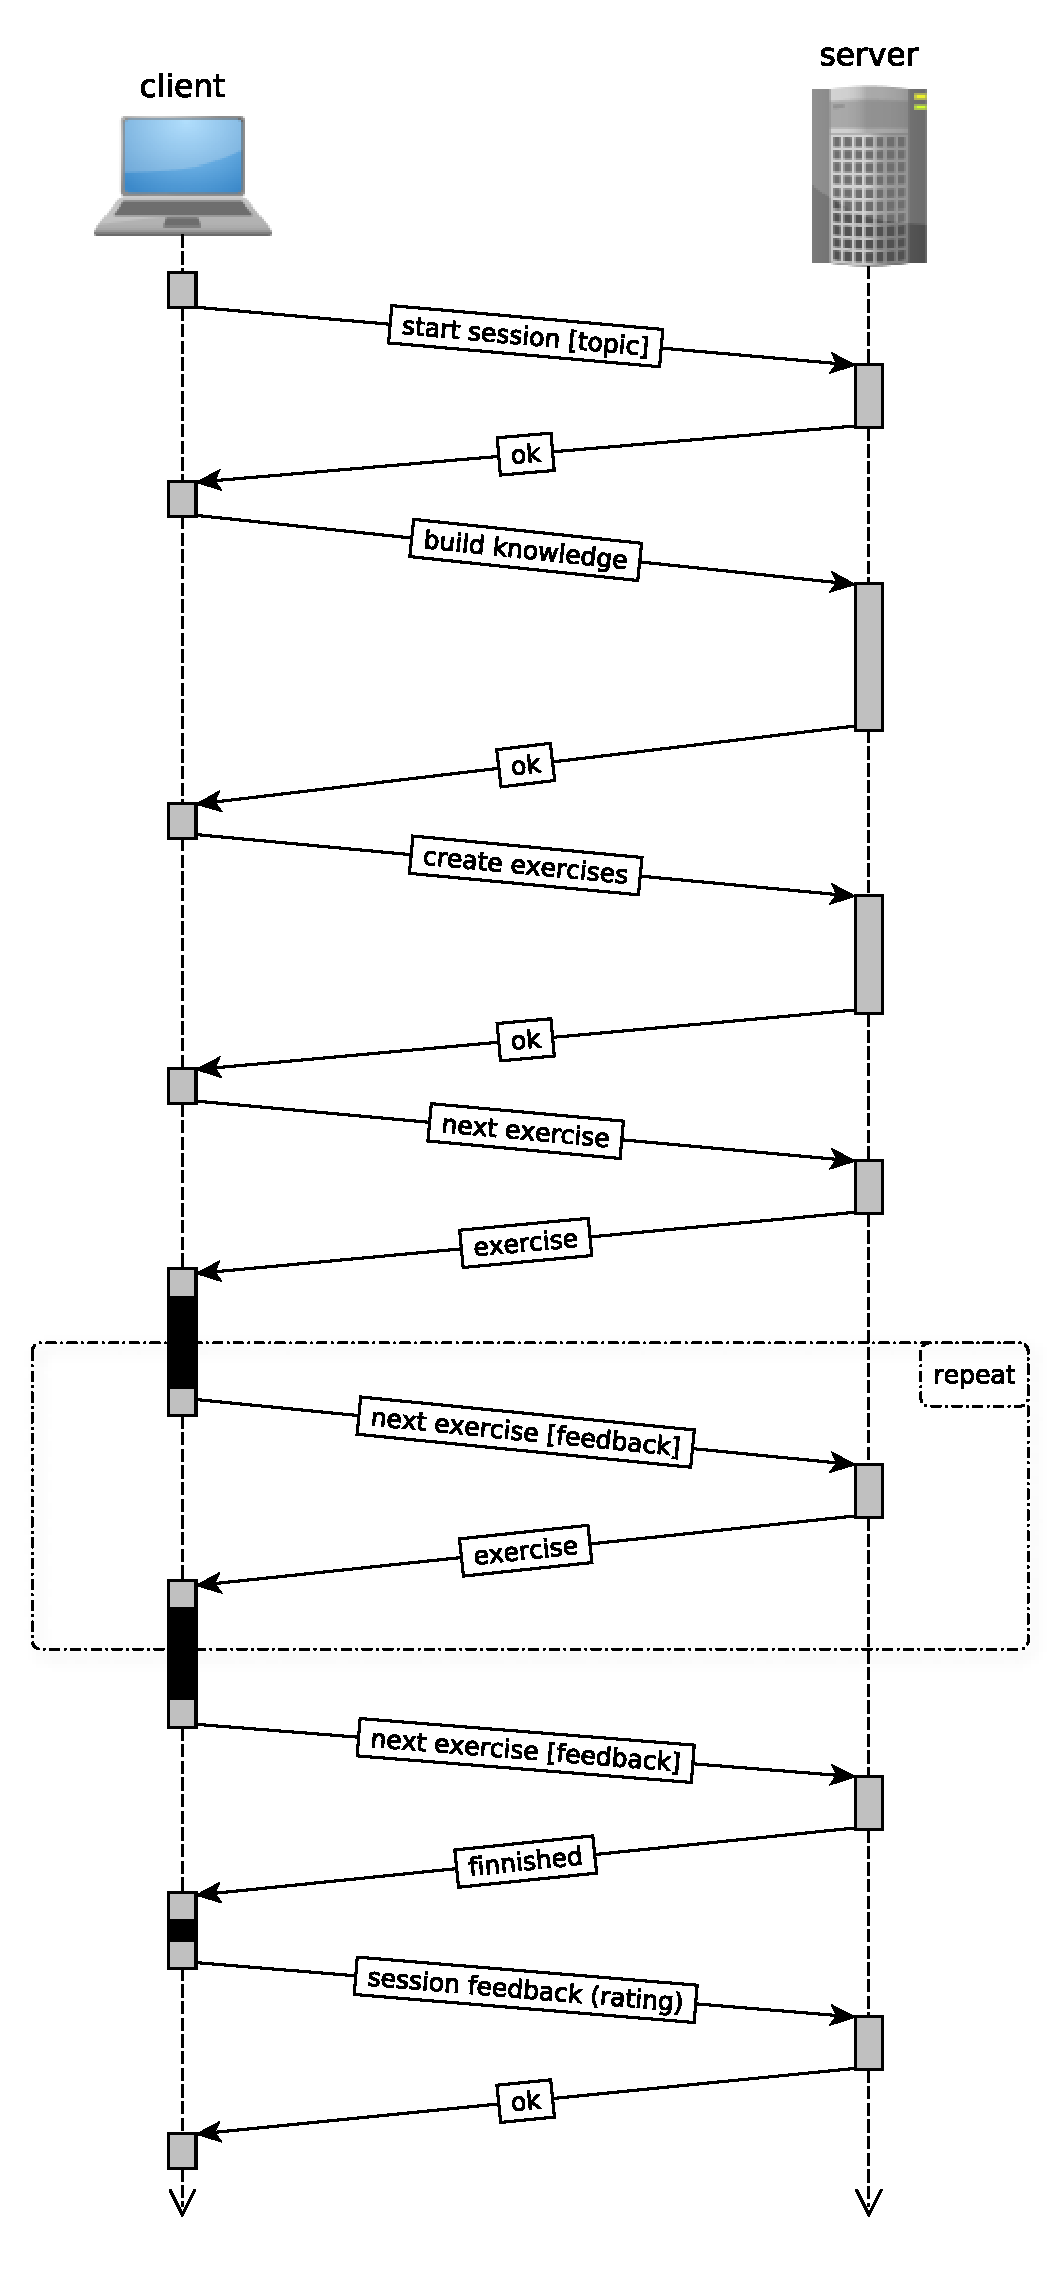
\includegraphics[width=0.66\textwidth]{images/client-server-communication.pdf}
  \caption{Client-server communication}
  \label{fig:client-server-communication}
\end{figure}


% ===========================  CHAPTER ===========================
\chapter{Deployment and Evaluation}
\label{chap:evaluation}

TODO: podrobnosti o nasazeni (server, db, virtualni prostredi, mozna nejake sturcne shrnuti potrebnych Pythonich knihoven)

TODO: vyhodnoceni jednotlivych komponent, (2 KB, 6 PR, a taky celkovy prumerny vykon): pocet ok otazek, a jaka byla skutecna uspesnost, prip. zpetne vazby, pokud nejake budou.

TODO: bylo by pekne, kdybych mohl ze ziskanych dat take zmerit RMSE tech 6 ruznych pracitce komponent (resp. te jejich casti, ktera modeluje studenta, tj. jak moc dobre ohdaduji, ze to uzivatel zvladne)


% ===========================  CHAPTER ===========================
\chapter{Conclusions and Future Plans}
\label{chap:future}

TODO: strucne shrnuti a hlavne zavery na zaklade statistik a strucne budouci plany...

TODO: what to improve (... in diploma thesis)

TODO: evolucni algoritmy pro hledani optimalnich parameteru (nebo i kodu!) komponent

TODO: nejaka ukazka zajimavejsiho cviceni

TODO: procist si sve napady z notes.txt v Procvicniku-v1





% ===== APPENDIX AND BIBLIOGRAPHY =====
\appendix

% include citations not cited specifically
%\nocite{*}

% print complete bibliography
\printbibliography

\chapter{Data attachment}

TODO: data attachment structure description

\end{document}
